% For more detailed article preparation guidelines, please see:
% http://f1000research.com/author-guidelines
\documentclass[10pt,a4paper,onecolumn]{article}
\usepackage{f1000_styles}
\usepackage{units}
\geometry{right=4cm}
% enable the 'endfloat' package to sort all tables and figures to the
% end of the document without having to edit the manuscript
%\usepackage{endfloat}
\usepackage{booktabs}
\usepackage[
	colorlinks=true,
	urlcolor=blue,
	linkcolor=green
]{hyperref}
%% Default: numerical citations
\usepackage[numbers]{natbib}

%% Uncomment this lines for superscript citations instead
% \usepackage[super]{natbib}

%% Uncomment these lines for author-year citations instead
% \usepackage[round]{natbib}
% \let\cite\citep

\begin{document}
% Overview
\newcommand{\SentencesRun0}{2528}
\newcommand{\SentencesRun1}{292}
\newcommand{\SentencesRun2}{366}
\newcommand{\SentencesRun3}{320}
\newcommand{\SentencesRun4}{352}
\newcommand{\SentencesRun5}{344}
\newcommand{\SentencesRun6}{289}
\newcommand{\SentencesRun7}{365}
\newcommand{\SentencesRun8}{200}

\newcommand{\WordsRun0}{16187}
\newcommand{\WordsRun1}{2089}
\newcommand{\WordsRun2}{2162}
\newcommand{\WordsRun3}{2115}
\newcommand{\WordsRun4}{2035}
\newcommand{\WordsRun5}{2217}
\newcommand{\WordsRun6}{2033}
\newcommand{\WordsRun7}{2322}
\newcommand{\WordsRun8}{1214}

\newcommand{\PhonesRun0}{66611}
\newcommand{\PhonesRun1}{8802}
\newcommand{\PhonesRun2}{8727}
\newcommand{\PhonesRun3}{8770}
\newcommand{\PhonesRun4}{8557}
\newcommand{\PhonesRun5}{9197}
\newcommand{\PhonesRun6}{8353}
\newcommand{\PhonesRun7}{9351}
\newcommand{\PhonesRun8}{4854}


% Sentences by Speaker
\newcommand{\BubbaRun0}{74}
\newcommand{\BubbaRun1}{0}
\newcommand{\BubbaRun2}{16}
\newcommand{\BubbaRun3}{40}
\newcommand{\BubbaRun4}{18}
\newcommand{\BubbaRun5}{0}
\newcommand{\BubbaRun6}{0}
\newcommand{\BubbaRun7}{0}
\newcommand{\BubbaRun8}{0}

\newcommand{\DrillsergeantRun0}{16}
\newcommand{\DrillsergeantRun1}{0}
\newcommand{\DrillsergeantRun2}{0}
\newcommand{\DrillsergeantRun3}{16}
\newcommand{\DrillsergeantRun4}{0}
\newcommand{\DrillsergeantRun5}{0}
\newcommand{\DrillsergeantRun6}{0}
\newcommand{\DrillsergeantRun7}{0}
\newcommand{\DrillsergeantRun8}{0}

\newcommand{\ForrestRun0}{354}
\newcommand{\ForrestRun1}{22}
\newcommand{\ForrestRun2}{37}
\newcommand{\ForrestRun3}{22}
\newcommand{\ForrestRun4}{48}
\newcommand{\ForrestRun5}{50}
\newcommand{\ForrestRun6}{61}
\newcommand{\ForrestRun7}{49}
\newcommand{\ForrestRun8}{65}

\newcommand{\ForrestchildRun0}{19}
\newcommand{\ForrestchildRun1}{17}
\newcommand{\ForrestchildRun2}{2}
\newcommand{\ForrestchildRun3}{0}
\newcommand{\ForrestchildRun4}{0}
\newcommand{\ForrestchildRun5}{0}
\newcommand{\ForrestchildRun6}{0}
\newcommand{\ForrestchildRun7}{0}
\newcommand{\ForrestchildRun8}{0}

\newcommand{\ForrestvoRun0}{369}
\newcommand{\ForrestvoRun1}{61}
\newcommand{\ForrestvoRun2}{48}
\newcommand{\ForrestvoRun3}{53}
\newcommand{\ForrestvoRun4}{51}
\newcommand{\ForrestvoRun5}{37}
\newcommand{\ForrestvoRun6}{40}
\newcommand{\ForrestvoRun7}{63}
\newcommand{\ForrestvoRun8}{16}

\newcommand{\JennyRun0}{177}
\newcommand{\JennyRun1}{0}
\newcommand{\JennyRun2}{46}
\newcommand{\JennyRun3}{30}
\newcommand{\JennyRun4}{3}
\newcommand{\JennyRun5}{25}
\newcommand{\JennyRun6}{0}
\newcommand{\JennyRun7}{57}
\newcommand{\JennyRun8}{16}

\newcommand{\JennychildRun0}{23}
\newcommand{\JennychildRun1}{7}
\newcommand{\JennychildRun2}{16}
\newcommand{\JennychildRun3}{0}
\newcommand{\JennychildRun4}{0}
\newcommand{\JennychildRun5}{0}
\newcommand{\JennychildRun6}{0}
\newcommand{\JennychildRun7}{0}
\newcommand{\JennychildRun8}{0}

\newcommand{\LtdanRun0}{183}
\newcommand{\LtdanRun1}{0}
\newcommand{\LtdanRun2}{0}
\newcommand{\LtdanRun3}{49}
\newcommand{\LtdanRun4}{33}
\newcommand{\LtdanRun5}{65}
\newcommand{\LtdanRun6}{28}
\newcommand{\LtdanRun7}{0}
\newcommand{\LtdanRun8}{8}

\newcommand{\MrsgumpRun0}{53}
\newcommand{\MrsgumpRun1}{38}
\newcommand{\MrsgumpRun2}{2}
\newcommand{\MrsgumpRun3}{0}
\newcommand{\MrsgumpRun4}{0}
\newcommand{\MrsgumpRun5}{0}
\newcommand{\MrsgumpRun6}{13}
\newcommand{\MrsgumpRun7}{0}
\newcommand{\MrsgumpRun8}{0}

\newcommand{\NarratorRun0}{903}
\newcommand{\NarratorRun1}{111}
\newcommand{\NarratorRun2}{134}
\newcommand{\NarratorRun3}{78}
\newcommand{\NarratorRun4}{139}
\newcommand{\NarratorRun5}{93}
\newcommand{\NarratorRun6}{115}
\newcommand{\NarratorRun7}{147}
\newcommand{\NarratorRun8}{86}


% POS-Tagging
\newcommand{\PosAdj}{adjective}
\newcommand{\PosAdjRun0}{916}
\newcommand{\PosAdjRun1}{138}
\newcommand{\PosAdjRun2}{126}
\newcommand{\PosAdjRun3}{106}
\newcommand{\PosAdjRun4}{96}
\newcommand{\PosAdjRun5}{130}
\newcommand{\PosAdjRun6}{118}
\newcommand{\PosAdjRun7}{128}
\newcommand{\PosAdjRun8}{74}

\newcommand{\PosAdp}{adposition}
\newcommand{\PosAdpRun0}{1429}
\newcommand{\PosAdpRun1}{181}
\newcommand{\PosAdpRun2}{176}
\newcommand{\PosAdpRun3}{176}
\newcommand{\PosAdpRun4}{194}
\newcommand{\PosAdpRun5}{188}
\newcommand{\PosAdpRun6}{183}
\newcommand{\PosAdpRun7}{213}
\newcommand{\PosAdpRun8}{118}

\newcommand{\PosAdv}{adverb}
\newcommand{\PosAdvRun0}{1332}
\newcommand{\PosAdvRun1}{166}
\newcommand{\PosAdvRun2}{169}
\newcommand{\PosAdvRun3}{220}
\newcommand{\PosAdvRun4}{162}
\newcommand{\PosAdvRun5}{178}
\newcommand{\PosAdvRun6}{169}
\newcommand{\PosAdvRun7}{193}
\newcommand{\PosAdvRun8}{75}

\newcommand{\PosAux}{auxiliary}
\newcommand{\PosAuxRun0}{807}
\newcommand{\PosAuxRun1}{102}
\newcommand{\PosAuxRun2}{120}
\newcommand{\PosAuxRun3}{92}
\newcommand{\PosAuxRun4}{96}
\newcommand{\PosAuxRun5}{125}
\newcommand{\PosAuxRun6}{110}
\newcommand{\PosAuxRun7}{112}
\newcommand{\PosAuxRun8}{50}

\newcommand{\PosConj}{conjunction}
\newcommand{\PosConjRun0}{525}
\newcommand{\PosConjRun1}{74}
\newcommand{\PosConjRun2}{63}
\newcommand{\PosConjRun3}{71}
\newcommand{\PosConjRun4}{49}
\newcommand{\PosConjRun5}{61}
\newcommand{\PosConjRun6}{80}
\newcommand{\PosConjRun7}{86}
\newcommand{\PosConjRun8}{41}

\newcommand{\PosDet}{determiner}
\newcommand{\PosDetRun0}{1754}
\newcommand{\PosDetRun1}{257}
\newcommand{\PosDetRun2}{243}
\newcommand{\PosDetRun3}{198}
\newcommand{\PosDetRun4}{219}
\newcommand{\PosDetRun5}{220}
\newcommand{\PosDetRun6}{222}
\newcommand{\PosDetRun7}{254}
\newcommand{\PosDetRun8}{141}

\newcommand{\PosNonspeechRun0}{202}
\newcommand{\PosNonspeechRun1}{23}
\newcommand{\PosNonspeechRun2}{21}
\newcommand{\PosNonspeechRun3}{9}
\newcommand{\PosNonspeechRun4}{23}
\newcommand{\PosNonspeechRun5}{55}
\newcommand{\PosNonspeechRun6}{44}
\newcommand{\PosNonspeechRun7}{13}
\newcommand{\PosNonspeechRun8}{14}

\newcommand{\PosNoun}{noun}
\newcommand{\PosNounRun0}{2620}
\newcommand{\PosNounRun1}{361}
\newcommand{\PosNounRun2}{341}
\newcommand{\PosNounRun3}{332}
\newcommand{\PosNounRun4}{343}
\newcommand{\PosNounRun5}{331}
\newcommand{\PosNounRun6}{356}
\newcommand{\PosNounRun7}{351}
\newcommand{\PosNounRun8}{205}

\newcommand{\PosNum}{numeral}
\newcommand{\PosNumRun0}{66}
\newcommand{\PosNumRun1}{8}
\newcommand{\PosNumRun2}{11}
\newcommand{\PosNumRun3}{11}
\newcommand{\PosNumRun4}{7}
\newcommand{\PosNumRun5}{4}
\newcommand{\PosNumRun6}{9}
\newcommand{\PosNumRun7}{14}
\newcommand{\PosNumRun8}{2}

\newcommand{\PosPart}{particle}
\newcommand{\PosPartRun0}{572}
\newcommand{\PosPartRun1}{60}
\newcommand{\PosPartRun2}{100}
\newcommand{\PosPartRun3}{90}
\newcommand{\PosPartRun4}{62}
\newcommand{\PosPartRun5}{83}
\newcommand{\PosPartRun6}{53}
\newcommand{\PosPartRun7}{86}
\newcommand{\PosPartRun8}{38}

\newcommand{\PosPron}{pronoun}
\newcommand{\PosPronRun0}{2348}
\newcommand{\PosPronRun1}{275}
\newcommand{\PosPronRun2}{321}
\newcommand{\PosPronRun3}{328}
\newcommand{\PosPronRun4}{260}
\newcommand{\PosPronRun5}{348}
\newcommand{\PosPronRun6}{262}
\newcommand{\PosPronRun7}{362}
\newcommand{\PosPronRun8}{192}

\newcommand{\PosPropn}{proper noun}
\newcommand{\PosPropnRun0}{1012}
\newcommand{\PosPropnRun1}{131}
\newcommand{\PosPropnRun2}{135}
\newcommand{\PosPropnRun3}{119}
\newcommand{\PosPropnRun4}{168}
\newcommand{\PosPropnRun5}{162}
\newcommand{\PosPropnRun6}{116}
\newcommand{\PosPropnRun7}{117}
\newcommand{\PosPropnRun8}{64}

\newcommand{\PosSconj}{subordinating conjunction}
\newcommand{\PosSconjRun0}{172}
\newcommand{\PosSconjRun1}{19}
\newcommand{\PosSconjRun2}{18}
\newcommand{\PosSconjRun3}{20}
\newcommand{\PosSconjRun4}{15}
\newcommand{\PosSconjRun5}{31}
\newcommand{\PosSconjRun6}{27}
\newcommand{\PosSconjRun7}{26}
\newcommand{\PosSconjRun8}{16}

\newcommand{\PosVerb}{verb}
\newcommand{\PosVerbRun0}{2317}
\newcommand{\PosVerbRun1}{285}
\newcommand{\PosVerbRun2}{308}
\newcommand{\PosVerbRun3}{320}
\newcommand{\PosVerbRun4}{319}
\newcommand{\PosVerbRun5}{289}
\newcommand{\PosVerbRun6}{274}
\newcommand{\PosVerbRun7}{349}
\newcommand{\PosVerbRun8}{173}

\newcommand{\PosX}{other}
\newcommand{\PosXRun0}{108}
\newcommand{\PosXRun1}{8}
\newcommand{\PosXRun2}{10}
\newcommand{\PosXRun3}{21}
\newcommand{\PosXRun4}{21}
\newcommand{\PosXRun5}{11}
\newcommand{\PosXRun6}{9}
\newcommand{\PosXRun7}{17}
\newcommand{\PosXRun8}{11}


% TAG-Tagging
\newcommand{\TagAdja}{adjective, attributive}
\newcommand{\TagAdjaRun0}{478}
\newcommand{\TagAdjaRun1}{73}
\newcommand{\TagAdjaRun2}{58}
\newcommand{\TagAdjaRun3}{58}
\newcommand{\TagAdjaRun4}{51}
\newcommand{\TagAdjaRun5}{77}
\newcommand{\TagAdjaRun6}{58}
\newcommand{\TagAdjaRun7}{70}
\newcommand{\TagAdjaRun8}{33}

\newcommand{\TagAdjd}{adjective, adverbial or predicative}
\newcommand{\TagAdjdRun0}{438}
\newcommand{\TagAdjdRun1}{65}
\newcommand{\TagAdjdRun2}{68}
\newcommand{\TagAdjdRun3}{48}
\newcommand{\TagAdjdRun4}{45}
\newcommand{\TagAdjdRun5}{53}
\newcommand{\TagAdjdRun6}{60}
\newcommand{\TagAdjdRun7}{58}
\newcommand{\TagAdjdRun8}{41}

\newcommand{\TagAdv}{adverb}
\newcommand{\TagAdvRun0}{1181}
\newcommand{\TagAdvRun1}{146}
\newcommand{\TagAdvRun2}{145}
\newcommand{\TagAdvRun3}{201}
\newcommand{\TagAdvRun4}{143}
\newcommand{\TagAdvRun5}{157}
\newcommand{\TagAdvRun6}{149}
\newcommand{\TagAdvRun7}{174}
\newcommand{\TagAdvRun8}{66}

\newcommand{\TagAppr}{preposition; circumposition left}
\newcommand{\TagApprRun0}{1192}
\newcommand{\TagApprRun1}{156}
\newcommand{\TagApprRun2}{146}
\newcommand{\TagApprRun3}{156}
\newcommand{\TagApprRun4}{152}
\newcommand{\TagApprRun5}{157}
\newcommand{\TagApprRun6}{150}
\newcommand{\TagApprRun7}{178}
\newcommand{\TagApprRun8}{97}

\newcommand{\TagArt}{definite or indefinite article}
\newcommand{\TagArtRun0}{1340}
\newcommand{\TagArtRun1}{199}
\newcommand{\TagArtRun2}{183}
\newcommand{\TagArtRun3}{140}
\newcommand{\TagArtRun4}{178}
\newcommand{\TagArtRun5}{159}
\newcommand{\TagArtRun6}{176}
\newcommand{\TagArtRun7}{191}
\newcommand{\TagArtRun8}{114}

\newcommand{\TagKon}{coordinate conjunction}
\newcommand{\TagKonRun0}{475}
\newcommand{\TagKonRun1}{58}
\newcommand{\TagKonRun2}{58}
\newcommand{\TagKonRun3}{66}
\newcommand{\TagKonRun4}{45}
\newcommand{\TagKonRun5}{58}
\newcommand{\TagKonRun6}{76}
\newcommand{\TagKonRun7}{78}
\newcommand{\TagKonRun8}{36}

\newcommand{\TagNe}{proper noun}
\newcommand{\TagNeRun0}{1012}
\newcommand{\TagNeRun1}{131}
\newcommand{\TagNeRun2}{135}
\newcommand{\TagNeRun3}{119}
\newcommand{\TagNeRun4}{168}
\newcommand{\TagNeRun5}{162}
\newcommand{\TagNeRun6}{116}
\newcommand{\TagNeRun7}{117}
\newcommand{\TagNeRun8}{64}

\newcommand{\TagNn}{noun, singular or mass}
\newcommand{\TagNnRun0}{2620}
\newcommand{\TagNnRun1}{361}
\newcommand{\TagNnRun2}{341}
\newcommand{\TagNnRun3}{332}
\newcommand{\TagNnRun4}{343}
\newcommand{\TagNnRun5}{331}
\newcommand{\TagNnRun6}{356}
\newcommand{\TagNnRun7}{351}
\newcommand{\TagNnRun8}{205}

\newcommand{\TagPper}{non-reflexive personal pronoun}
\newcommand{\TagPperRun0}{1638}
\newcommand{\TagPperRun1}{183}
\newcommand{\TagPperRun2}{210}
\newcommand{\TagPperRun3}{221}
\newcommand{\TagPperRun4}{168}
\newcommand{\TagPperRun5}{246}
\newcommand{\TagPperRun6}{176}
\newcommand{\TagPperRun7}{287}
\newcommand{\TagPperRun8}{147}

\newcommand{\TagPposat}{attributive possessive pronoun}
\newcommand{\TagPposatRun0}{274}
\newcommand{\TagPposatRun1}{34}
\newcommand{\TagPposatRun2}{47}
\newcommand{\TagPposatRun3}{36}
\newcommand{\TagPposatRun4}{23}
\newcommand{\TagPposatRun5}{39}
\newcommand{\TagPposatRun6}{32}
\newcommand{\TagPposatRun7}{40}
\newcommand{\TagPposatRun8}{23}

\newcommand{\TagPtkvz}{separable verbal particle}
\newcommand{\TagPtkvzRun0}{353}
\newcommand{\TagPtkvzRun1}{34}
\newcommand{\TagPtkvzRun2}{63}
\newcommand{\TagPtkvzRun3}{49}
\newcommand{\TagPtkvzRun4}{46}
\newcommand{\TagPtkvzRun5}{41}
\newcommand{\TagPtkvzRun6}{33}
\newcommand{\TagPtkvzRun7}{60}
\newcommand{\TagPtkvzRun8}{27}

\newcommand{\TagVafin}{finite verb, auxiliary}
\newcommand{\TagVafinRun0}{767}
\newcommand{\TagVafinRun1}{96}
\newcommand{\TagVafinRun2}{108}
\newcommand{\TagVafinRun3}{89}
\newcommand{\TagVafinRun4}{92}
\newcommand{\TagVafinRun5}{116}
\newcommand{\TagVafinRun6}{106}
\newcommand{\TagVafinRun7}{110}
\newcommand{\TagVafinRun8}{50}

\newcommand{\TagVvfin}{finite verb, full}
\newcommand{\TagVvfinRun0}{1512}
\newcommand{\TagVvfinRun1}{181}
\newcommand{\TagVvfinRun2}{213}
\newcommand{\TagVvfinRun3}{201}
\newcommand{\TagVvfinRun4}{202}
\newcommand{\TagVvfinRun5}{172}
\newcommand{\TagVvfinRun6}{181}
\newcommand{\TagVvfinRun7}{228}
\newcommand{\TagVvfinRun8}{134}

\newcommand{\TagVvinf}{infinitive, full}
\newcommand{\TagVvinfRun0}{271}
\newcommand{\TagVvinfRun1}{37}
\newcommand{\TagVvinfRun2}{25}
\newcommand{\TagVvinfRun3}{51}
\newcommand{\TagVvinfRun4}{32}
\newcommand{\TagVvinfRun5}{42}
\newcommand{\TagVvinfRun6}{27}
\newcommand{\TagVvinfRun7}{40}
\newcommand{\TagVvinfRun8}{17}

\newcommand{\TagVvpp}{perfect participle, full}
\newcommand{\TagVvppRun0}{329}
\newcommand{\TagVvppRun1}{37}
\newcommand{\TagVvppRun2}{40}
\newcommand{\TagVvppRun3}{35}
\newcommand{\TagVvppRun4}{58}
\newcommand{\TagVvppRun5}{44}
\newcommand{\TagVvppRun6}{51}
\newcommand{\TagVvppRun7}{50}
\newcommand{\TagVvppRun8}{14}


% Syntactic Dependencies
\newcommand{\DepRootRun0}{2417}
\newcommand{\DepRootRun1}{285}
\newcommand{\DepRootRun2}{349}
\newcommand{\DepRootRun3}{322}
\newcommand{\DepRootRun4}{336}
\newcommand{\DepRootRun5}{317}
\newcommand{\DepRootRun6}{267}
\newcommand{\DepRootRun7}{358}
\newcommand{\DepRootRun8}{183}

\newcommand{\DepCd}{coordinating conjunction}
\newcommand{\DepCdRun0}{335}
\newcommand{\DepCdRun1}{48}
\newcommand{\DepCdRun2}{44}
\newcommand{\DepCdRun3}{48}
\newcommand{\DepCdRun4}{34}
\newcommand{\DepCdRun5}{41}
\newcommand{\DepCdRun6}{53}
\newcommand{\DepCdRun7}{42}
\newcommand{\DepCdRun8}{25}

\newcommand{\DepCj}{conjunct}
\newcommand{\DepCjRun0}{524}
\newcommand{\DepCjRun1}{65}
\newcommand{\DepCjRun2}{74}
\newcommand{\DepCjRun3}{88}
\newcommand{\DepCjRun4}{53}
\newcommand{\DepCjRun5}{65}
\newcommand{\DepCjRun6}{80}
\newcommand{\DepCjRun7}{65}
\newcommand{\DepCjRun8}{34}

\newcommand{\DepCp}{complementizer}
\newcommand{\DepCpRun0}{160}
\newcommand{\DepCpRun1}{17}
\newcommand{\DepCpRun2}{17}
\newcommand{\DepCpRun3}{20}
\newcommand{\DepCpRun4}{16}
\newcommand{\DepCpRun5}{29}
\newcommand{\DepCpRun6}{25}
\newcommand{\DepCpRun7}{21}
\newcommand{\DepCpRun8}{15}

\newcommand{\DepDa}{dative}
\newcommand{\DepDaRun0}{170}
\newcommand{\DepDaRun1}{15}
\newcommand{\DepDaRun2}{30}
\newcommand{\DepDaRun3}{27}
\newcommand{\DepDaRun4}{19}
\newcommand{\DepDaRun5}{23}
\newcommand{\DepDaRun6}{18}
\newcommand{\DepDaRun7}{27}
\newcommand{\DepDaRun8}{11}

\newcommand{\DepJu}{junctor}
\newcommand{\DepJuRun0}{130}
\newcommand{\DepJuRun1}{10}
\newcommand{\DepJuRun2}{13}
\newcommand{\DepJuRun3}{16}
\newcommand{\DepJuRun4}{12}
\newcommand{\DepJuRun5}{16}
\newcommand{\DepJuRun6}{22}
\newcommand{\DepJuRun7}{31}
\newcommand{\DepJuRun8}{10}

\newcommand{\DepMnr}{postnominal modifier}
\newcommand{\DepMnrRun0}{245}
\newcommand{\DepMnrRun1}{30}
\newcommand{\DepMnrRun2}{29}
\newcommand{\DepMnrRun3}{33}
\newcommand{\DepMnrRun4}{44}
\newcommand{\DepMnrRun5}{31}
\newcommand{\DepMnrRun6}{28}
\newcommand{\DepMnrRun7}{27}
\newcommand{\DepMnrRun8}{23}

\newcommand{\DepMo}{modifier}
\newcommand{\DepMoRun0}{2634}
\newcommand{\DepMoRun1}{349}
\newcommand{\DepMoRun2}{345}
\newcommand{\DepMoRun3}{355}
\newcommand{\DepMoRun4}{327}
\newcommand{\DepMoRun5}{356}
\newcommand{\DepMoRun6}{334}
\newcommand{\DepMoRun7}{384}
\newcommand{\DepMoRun8}{184}

\newcommand{\DepNk}{noun kernel element}
\newcommand{\DepNkRun0}{3763}
\newcommand{\DepNkRun1}{516}
\newcommand{\DepNkRun2}{482}
\newcommand{\DepNkRun3}{448}
\newcommand{\DepNkRun4}{475}
\newcommand{\DepNkRun5}{507}
\newcommand{\DepNkRun6}{485}
\newcommand{\DepNkRun7}{551}
\newcommand{\DepNkRun8}{299}

\newcommand{\DepOa}{accusative object}
\newcommand{\DepOaRun0}{1036}
\newcommand{\DepOaRun1}{117}
\newcommand{\DepOaRun2}{139}
\newcommand{\DepOaRun3}{149}
\newcommand{\DepOaRun4}{148}
\newcommand{\DepOaRun5}{146}
\newcommand{\DepOaRun6}{126}
\newcommand{\DepOaRun7}{134}
\newcommand{\DepOaRun8}{77}

\newcommand{\DepOc}{clausal object}
\newcommand{\DepOcRun0}{732}
\newcommand{\DepOcRun1}{98}
\newcommand{\DepOcRun2}{86}
\newcommand{\DepOcRun3}{97}
\newcommand{\DepOcRun4}{94}
\newcommand{\DepOcRun5}{105}
\newcommand{\DepOcRun6}{97}
\newcommand{\DepOcRun7}{115}
\newcommand{\DepOcRun8}{40}

\newcommand{\DepPd}{predicate}
\newcommand{\DepPdRun0}{301}
\newcommand{\DepPdRun1}{39}
\newcommand{\DepPdRun2}{50}
\newcommand{\DepPdRun3}{40}
\newcommand{\DepPdRun4}{25}
\newcommand{\DepPdRun5}{45}
\newcommand{\DepPdRun6}{41}
\newcommand{\DepPdRun7}{38}
\newcommand{\DepPdRun8}{23}

\newcommand{\DepPnc}{proper noun component}
\newcommand{\DepPncRun0}{154}
\newcommand{\DepPncRun1}{36}
\newcommand{\DepPncRun2}{19}
\newcommand{\DepPncRun3}{15}
\newcommand{\DepPncRun4}{14}
\newcommand{\DepPncRun5}{28}
\newcommand{\DepPncRun6}{22}
\newcommand{\DepPncRun7}{15}
\newcommand{\DepPncRun8}{5}

\newcommand{\DepSb}{subject}
\newcommand{\DepSbRun0}{2231}
\newcommand{\DepSbRun1}{280}
\newcommand{\DepSbRun2}{306}
\newcommand{\DepSbRun3}{271}
\newcommand{\DepSbRun4}{276}
\newcommand{\DepSbRun5}{301}
\newcommand{\DepSbRun6}{281}
\newcommand{\DepSbRun7}{340}
\newcommand{\DepSbRun8}{176}

\newcommand{\DepSvpRun0}{355}
\newcommand{\DepSvpRun1}{36}
\newcommand{\DepSvpRun2}{65}
\newcommand{\DepSvpRun3}{45}
\newcommand{\DepSvpRun4}{49}
\newcommand{\DepSvpRun5}{43}
\newcommand{\DepSvpRun6}{33}
\newcommand{\DepSvpRun7}{56}
\newcommand{\DepSvpRun8}{28}


% Descriptive Nouns
\newcommand{\DescrRun0}{17}
\newcommand{\DescrRun1}{2}
\newcommand{\DescrRun2}{2}
\newcommand{\DescrRun3}{2}
\newcommand{\DescrRun4}{0}
\newcommand{\DescrRun5}{3}
\newcommand{\DescrRun6}{3}
\newcommand{\DescrRun7}{4}
\newcommand{\DescrRun8}{1}

\newcommand{\DescrBodyRun0}{66}
\newcommand{\DescrBodyRun1}{6}
\newcommand{\DescrBodyRun2}{12}
\newcommand{\DescrBodyRun3}{7}
\newcommand{\DescrBodyRun4}{12}
\newcommand{\DescrBodyRun5}{2}
\newcommand{\DescrBodyRun6}{9}
\newcommand{\DescrBodyRun7}{13}
\newcommand{\DescrBodyRun8}{5}

\newcommand{\DescrBodypartRun0}{69}
\newcommand{\DescrBodypartRun1}{9}
\newcommand{\DescrBodypartRun2}{8}
\newcommand{\DescrBodypartRun3}{6}
\newcommand{\DescrBodypartRun4}{13}
\newcommand{\DescrBodypartRun5}{5}
\newcommand{\DescrBodypartRun6}{7}
\newcommand{\DescrBodypartRun7}{11}
\newcommand{\DescrBodypartRun8}{10}

\newcommand{\DescrFaceRun0}{47}
\newcommand{\DescrFaceRun1}{7}
\newcommand{\DescrFaceRun2}{7}
\newcommand{\DescrFaceRun3}{6}
\newcommand{\DescrFaceRun4}{1}
\newcommand{\DescrFaceRun5}{7}
\newcommand{\DescrFaceRun6}{9}
\newcommand{\DescrFaceRun7}{6}
\newcommand{\DescrFaceRun8}{4}

\newcommand{\DescrFemaleRun0}{31}
\newcommand{\DescrFemaleRun1}{12}
\newcommand{\DescrFemaleRun2}{8}
\newcommand{\DescrFemaleRun3}{0}
\newcommand{\DescrFemaleRun4}{3}
\newcommand{\DescrFemaleRun5}{0}
\newcommand{\DescrFemaleRun6}{3}
\newcommand{\DescrFemaleRun7}{2}
\newcommand{\DescrFemaleRun8}{3}

\newcommand{\DescrFemalesRun0}{3}
\newcommand{\DescrFemalesRun1}{0}
\newcommand{\DescrFemalesRun2}{0}
\newcommand{\DescrFemalesRun3}{0}
\newcommand{\DescrFemalesRun4}{2}
\newcommand{\DescrFemalesRun5}{0}
\newcommand{\DescrFemalesRun6}{0}
\newcommand{\DescrFemalesRun7}{1}
\newcommand{\DescrFemalesRun8}{0}

\newcommand{\DescrFnameRun0}{74}
\newcommand{\DescrFnameRun1}{2}
\newcommand{\DescrFnameRun2}{14}
\newcommand{\DescrFnameRun3}{6}
\newcommand{\DescrFnameRun4}{1}
\newcommand{\DescrFnameRun5}{13}
\newcommand{\DescrFnameRun6}{7}
\newcommand{\DescrFnameRun7}{20}
\newcommand{\DescrFnameRun8}{11}

\newcommand{\DescrFurnitureRun0}{50}
\newcommand{\DescrFurnitureRun1}{8}
\newcommand{\DescrFurnitureRun2}{5}
\newcommand{\DescrFurnitureRun3}{2}
\newcommand{\DescrFurnitureRun4}{5}
\newcommand{\DescrFurnitureRun5}{7}
\newcommand{\DescrFurnitureRun6}{10}
\newcommand{\DescrFurnitureRun7}{7}
\newcommand{\DescrFurnitureRun8}{6}

\newcommand{\DescrGeoRun0}{125}
\newcommand{\DescrGeoRun1}{16}
\newcommand{\DescrGeoRun2}{17}
\newcommand{\DescrGeoRun3}{11}
\newcommand{\DescrGeoRun4}{32}
\newcommand{\DescrGeoRun5}{0}
\newcommand{\DescrGeoRun6}{15}
\newcommand{\DescrGeoRun7}{18}
\newcommand{\DescrGeoRun8}{16}

\newcommand{\DescrGeoroomRun0}{105}
\newcommand{\DescrGeoroomRun1}{12}
\newcommand{\DescrGeoroomRun2}{11}
\newcommand{\DescrGeoroomRun3}{8}
\newcommand{\DescrGeoroomRun4}{5}
\newcommand{\DescrGeoroomRun5}{8}
\newcommand{\DescrGeoroomRun6}{25}
\newcommand{\DescrGeoroomRun7}{28}
\newcommand{\DescrGeoroomRun8}{8}

\newcommand{\DescrHeadRun0}{36}
\newcommand{\DescrHeadRun1}{5}
\newcommand{\DescrHeadRun2}{4}
\newcommand{\DescrHeadRun3}{4}
\newcommand{\DescrHeadRun4}{4}
\newcommand{\DescrHeadRun5}{2}
\newcommand{\DescrHeadRun6}{4}
\newcommand{\DescrHeadRun7}{6}
\newcommand{\DescrHeadRun8}{7}

\newcommand{\DescrMaleRun0}{89}
\newcommand{\DescrMaleRun1}{15}
\newcommand{\DescrMaleRun2}{18}
\newcommand{\DescrMaleRun3}{9}
\newcommand{\DescrMaleRun4}{18}
\newcommand{\DescrMaleRun5}{7}
\newcommand{\DescrMaleRun6}{8}
\newcommand{\DescrMaleRun7}{9}
\newcommand{\DescrMaleRun8}{5}

\newcommand{\DescrMalesRun0}{23}
\newcommand{\DescrMalesRun1}{2}
\newcommand{\DescrMalesRun2}{11}
\newcommand{\DescrMalesRun3}{4}
\newcommand{\DescrMalesRun4}{3}
\newcommand{\DescrMalesRun5}{2}
\newcommand{\DescrMalesRun6}{0}
\newcommand{\DescrMalesRun7}{1}
\newcommand{\DescrMalesRun8}{0}

\newcommand{\DescrMnameRun0}{291}
\newcommand{\DescrMnameRun1}{24}
\newcommand{\DescrMnameRun2}{39}
\newcommand{\DescrMnameRun3}{25}
\newcommand{\DescrMnameRun4}{81}
\newcommand{\DescrMnameRun5}{36}
\newcommand{\DescrMnameRun6}{34}
\newcommand{\DescrMnameRun7}{32}
\newcommand{\DescrMnameRun8}{20}

\newcommand{\DescrObjectRun0}{232}
\newcommand{\DescrObjectRun1}{36}
\newcommand{\DescrObjectRun2}{22}
\newcommand{\DescrObjectRun3}{20}
\newcommand{\DescrObjectRun4}{30}
\newcommand{\DescrObjectRun5}{25}
\newcommand{\DescrObjectRun6}{37}
\newcommand{\DescrObjectRun7}{26}
\newcommand{\DescrObjectRun8}{36}

\newcommand{\DescrObjectsRun0}{52}
\newcommand{\DescrObjectsRun1}{3}
\newcommand{\DescrObjectsRun2}{12}
\newcommand{\DescrObjectsRun3}{7}
\newcommand{\DescrObjectsRun4}{14}
\newcommand{\DescrObjectsRun5}{4}
\newcommand{\DescrObjectsRun6}{5}
\newcommand{\DescrObjectsRun7}{6}
\newcommand{\DescrObjectsRun8}{1}

\newcommand{\DescrPersonsRun0}{17}
\newcommand{\DescrPersonsRun1}{0}
\newcommand{\DescrPersonsRun2}{3}
\newcommand{\DescrPersonsRun3}{1}
\newcommand{\DescrPersonsRun4}{2}
\newcommand{\DescrPersonsRun5}{3}
\newcommand{\DescrPersonsRun6}{1}
\newcommand{\DescrPersonsRun7}{5}
\newcommand{\DescrPersonsRun8}{2}

\newcommand{\DescrSettingnewRun0}{86}
\newcommand{\DescrSettingnewRun1}{11}
\newcommand{\DescrSettingnewRun2}{15}
\newcommand{\DescrSettingnewRun3}{12}
\newcommand{\DescrSettingnewRun4}{4}
\newcommand{\DescrSettingnewRun5}{15}
\newcommand{\DescrSettingnewRun6}{10}
\newcommand{\DescrSettingnewRun7}{16}
\newcommand{\DescrSettingnewRun8}{3}

\newcommand{\DescrSettingrecRun0}{37}
\newcommand{\DescrSettingrecRun1}{2}
\newcommand{\DescrSettingrecRun2}{5}
\newcommand{\DescrSettingrecRun3}{1}
\newcommand{\DescrSettingrecRun4}{4}
\newcommand{\DescrSettingrecRun5}{2}
\newcommand{\DescrSettingrecRun6}{9}
\newcommand{\DescrSettingrecRun7}{8}
\newcommand{\DescrSettingrecRun8}{6}


\newcommand{\AdjaRun0}{478}
\newcommand{\AdjaRun1}{73}
\newcommand{\AdjaRun2}{58}
\newcommand{\AdjaRun3}{58}
\newcommand{\AdjaRun4}{51}
\newcommand{\AdjaRun5}{77}
\newcommand{\AdjaRun6}{58}
\newcommand{\AdjaRun7}{70}
\newcommand{\AdjaRun8}{33}

\newcommand{\AdjdRun0}{438}
\newcommand{\AdjdRun1}{65}
\newcommand{\AdjdRun2}{68}
\newcommand{\AdjdRun3}{48}
\newcommand{\AdjdRun4}{45}
\newcommand{\AdjdRun5}{53}
\newcommand{\AdjdRun6}{60}
\newcommand{\AdjdRun7}{58}
\newcommand{\AdjdRun8}{41}

\newcommand{\AdvRun0}{1181}
\newcommand{\AdvRun1}{146}
\newcommand{\AdvRun2}{145}
\newcommand{\AdvRun3}{201}
\newcommand{\AdvRun4}{143}
\newcommand{\AdvRun5}{157}
\newcommand{\AdvRun6}{149}
\newcommand{\AdvRun7}{174}
\newcommand{\AdvRun8}{66}

\newcommand{\ApprRun0}{1192}
\newcommand{\ApprRun1}{156}
\newcommand{\ApprRun2}{146}
\newcommand{\ApprRun3}{156}
\newcommand{\ApprRun4}{152}
\newcommand{\ApprRun5}{157}
\newcommand{\ApprRun6}{150}
\newcommand{\ApprRun7}{178}
\newcommand{\ApprRun8}{97}

\newcommand{\ApprartRun0}{233}
\newcommand{\ApprartRun1}{24}
\newcommand{\ApprartRun2}{28}
\newcommand{\ApprartRun3}{20}
\newcommand{\ApprartRun4}{42}
\newcommand{\ApprartRun5}{31}
\newcommand{\ApprartRun6}{32}
\newcommand{\ApprartRun7}{35}
\newcommand{\ApprartRun8}{21}

\newcommand{\ArtRun0}{1340}
\newcommand{\ArtRun1}{199}
\newcommand{\ArtRun2}{183}
\newcommand{\ArtRun3}{140}
\newcommand{\ArtRun4}{178}
\newcommand{\ArtRun5}{159}
\newcommand{\ArtRun6}{176}
\newcommand{\ArtRun7}{191}
\newcommand{\ArtRun8}{114}

\newcommand{\Fg_ad_lrdiffRun0}{180133}
\newcommand{\Fg_ad_lrdiffRun1}{22574}
\newcommand{\Fg_ad_lrdiffRun2}{22075}
\newcommand{\Fg_ad_lrdiffRun3}{21925}
\newcommand{\Fg_ad_lrdiffRun4}{24425}
\newcommand{\Fg_ad_lrdiffRun5}{23125}
\newcommand{\Fg_ad_lrdiffRun6}{21975}
\newcommand{\Fg_ad_lrdiffRun7}{27175}
\newcommand{\Fg_ad_lrdiffRun8}{16859}

\newcommand{\Fg_ad_rmsRun0}{180133}
\newcommand{\Fg_ad_rmsRun1}{22574}
\newcommand{\Fg_ad_rmsRun2}{22075}
\newcommand{\Fg_ad_rmsRun3}{21925}
\newcommand{\Fg_ad_rmsRun4}{24425}
\newcommand{\Fg_ad_rmsRun5}{23125}
\newcommand{\Fg_ad_rmsRun6}{21975}
\newcommand{\Fg_ad_rmsRun7}{27175}
\newcommand{\Fg_ad_rmsRun8}{16859}

\newcommand{\KonRun0}{475}
\newcommand{\KonRun1}{58}
\newcommand{\KonRun2}{58}
\newcommand{\KonRun3}{66}
\newcommand{\KonRun4}{45}
\newcommand{\KonRun5}{58}
\newcommand{\KonRun6}{76}
\newcommand{\KonRun7}{78}
\newcommand{\KonRun8}{36}

\newcommand{\NeRun0}{1012}
\newcommand{\NeRun1}{131}
\newcommand{\NeRun2}{135}
\newcommand{\NeRun3}{119}
\newcommand{\NeRun4}{168}
\newcommand{\NeRun5}{162}
\newcommand{\NeRun6}{116}
\newcommand{\NeRun7}{117}
\newcommand{\NeRun8}{64}

\newcommand{\NnRun0}{2620}
\newcommand{\NnRun1}{361}
\newcommand{\NnRun2}{341}
\newcommand{\NnRun3}{332}
\newcommand{\NnRun4}{343}
\newcommand{\NnRun5}{331}
\newcommand{\NnRun6}{356}
\newcommand{\NnRun7}{351}
\newcommand{\NnRun8}{205}

\newcommand{\No-spRun0}{264}
\newcommand{\No-spRun1}{16}
\newcommand{\No-spRun2}{20}
\newcommand{\No-spRun3}{23}
\newcommand{\No-spRun4}{50}
\newcommand{\No-spRun5}{25}
\newcommand{\No-spRun6}{27}
\newcommand{\No-spRun7}{56}
\newcommand{\No-spRun8}{47}

\newcommand{\PdsRun0}{192}
\newcommand{\PdsRun1}{16}
\newcommand{\PdsRun2}{32}
\newcommand{\PdsRun3}{31}
\newcommand{\PdsRun4}{25}
\newcommand{\PdsRun5}{33}
\newcommand{\PdsRun6}{27}
\newcommand{\PdsRun7}{17}
\newcommand{\PdsRun8}{11}

\newcommand{\PhonesRun0}{65251}
\newcommand{\PhonesRun1}{8589}
\newcommand{\PhonesRun2}{8534}
\newcommand{\PhonesRun3}{8597}
\newcommand{\PhonesRun4}{8387}
\newcommand{\PhonesRun5}{8976}
\newcommand{\PhonesRun6}{8184}
\newcommand{\PhonesRun7}{9232}
\newcommand{\PhonesRun8}{4752}

\newcommand{\PisRun0}{217}
\newcommand{\PisRun1}{36}
\newcommand{\PisRun2}{30}
\newcommand{\PisRun3}{35}
\newcommand{\PisRun4}{28}
\newcommand{\PisRun5}{30}
\newcommand{\PisRun6}{21}
\newcommand{\PisRun7}{23}
\newcommand{\PisRun8}{14}

\newcommand{\PperRun0}{1638}
\newcommand{\PperRun1}{183}
\newcommand{\PperRun2}{210}
\newcommand{\PperRun3}{221}
\newcommand{\PperRun4}{168}
\newcommand{\PperRun5}{246}
\newcommand{\PperRun6}{176}
\newcommand{\PperRun7}{287}
\newcommand{\PperRun8}{147}

\newcommand{\PposatRun0}{274}
\newcommand{\PposatRun1}{34}
\newcommand{\PposatRun2}{47}
\newcommand{\PposatRun3}{36}
\newcommand{\PposatRun4}{23}
\newcommand{\PposatRun5}{39}
\newcommand{\PposatRun6}{32}
\newcommand{\PposatRun7}{40}
\newcommand{\PposatRun8}{23}

\newcommand{\PrfRun0}{157}
\newcommand{\PrfRun1}{18}
\newcommand{\PrfRun2}{25}
\newcommand{\PrfRun3}{15}
\newcommand{\PrfRun4}{23}
\newcommand{\PrfRun5}{17}
\newcommand{\PrfRun6}{26}
\newcommand{\PrfRun7}{19}
\newcommand{\PrfRun8}{14}

\newcommand{\PtkvzRun0}{353}
\newcommand{\PtkvzRun1}{34}
\newcommand{\PtkvzRun2}{63}
\newcommand{\PtkvzRun3}{49}
\newcommand{\PtkvzRun4}{46}
\newcommand{\PtkvzRun5}{41}
\newcommand{\PtkvzRun6}{33}
\newcommand{\PtkvzRun7}{60}
\newcommand{\PtkvzRun8}{27}

\newcommand{\SentenceRun0}{1651}
\newcommand{\SentenceRun1}{205}
\newcommand{\SentenceRun2}{231}
\newcommand{\SentenceRun3}{200}
\newcommand{\SentenceRun4}{215}
\newcommand{\SentenceRun5}{212}
\newcommand{\SentenceRun6}{198}
\newcommand{\SentenceRun7}{249}
\newcommand{\SentenceRun8}{141}

\newcommand{\Tag_otherRun0}{1123}
\newcommand{\Tag_otherRun1}{153}
\newcommand{\Tag_otherRun2}{165}
\newcommand{\Tag_otherRun3}{174}
\newcommand{\Tag_otherRun4}{124}
\newcommand{\Tag_otherRun5}{169}
\newcommand{\Tag_otherRun6}{121}
\newcommand{\Tag_otherRun7}{153}
\newcommand{\Tag_otherRun8}{64}

\newcommand{\VafinRun0}{767}
\newcommand{\VafinRun1}{96}
\newcommand{\VafinRun2}{108}
\newcommand{\VafinRun3}{89}
\newcommand{\VafinRun4}{92}
\newcommand{\VafinRun5}{116}
\newcommand{\VafinRun6}{106}
\newcommand{\VafinRun7}{110}
\newcommand{\VafinRun8}{50}

\newcommand{\VmfinRun0}{183}
\newcommand{\VmfinRun1}{28}
\newcommand{\VmfinRun2}{21}
\newcommand{\VmfinRun3}{29}
\newcommand{\VmfinRun4}{24}
\newcommand{\VmfinRun5}{28}
\newcommand{\VmfinRun6}{15}
\newcommand{\VmfinRun7}{30}
\newcommand{\VmfinRun8}{8}

\newcommand{\VvfinRun0}{1512}
\newcommand{\VvfinRun1}{181}
\newcommand{\VvfinRun2}{213}
\newcommand{\VvfinRun3}{201}
\newcommand{\VvfinRun4}{202}
\newcommand{\VvfinRun5}{172}
\newcommand{\VvfinRun6}{181}
\newcommand{\VvfinRun7}{228}
\newcommand{\VvfinRun8}{134}

\newcommand{\VvinfRun0}{271}
\newcommand{\VvinfRun1}{37}
\newcommand{\VvinfRun2}{25}
\newcommand{\VvinfRun3}{51}
\newcommand{\VvinfRun4}{32}
\newcommand{\VvinfRun5}{42}
\newcommand{\VvinfRun6}{27}
\newcommand{\VvinfRun7}{40}
\newcommand{\VvinfRun8}{17}

\newcommand{\VvppRun0}{329}
\newcommand{\VvppRun1}{37}
\newcommand{\VvppRun2}{40}
\newcommand{\VvppRun3}{35}
\newcommand{\VvppRun4}{58}
\newcommand{\VvppRun5}{44}
\newcommand{\VvppRun6}{51}
\newcommand{\VvppRun7}{50}
\newcommand{\VvppRun8}{14}



\title{A studyforrest extension, an annotation of spoken language in the German dubbed movie ``Forrest Gump'' and its audio-description}
%\titlenote{whatever titlenote here}

\author[1, 2]{Christian~O.~Häusler \\ email \href{mailto:c.haeusler@fz-juelich.de}{c.haeusler@fz-juelich.de} }
\author[1, 2]{Michael~Hanke \\ email \href{mailto:m.hanke@fz-juelich.de}{m.hanke@fz-juelich.de} }

\affil[1]{Institute of Neuroscience and Medicine, Brain \& Behaviour (INM-7), Research Centre Jülich, Jülich, 52425, Germany}
\affil[2]{Institute of Systems Neuroscience, Medical Faculty, Heinrich Heine University, Düsseldorf, 40225, Germany}

\maketitle

\todo[inline]{wie email und ORCID (du: https://orcid.org/0000-0001-6398-6370; ich: https://orcid.org/0000-0002-0936-317X) unterbringen?}

\todo{Wort zur Validierungsstudie; Es sind erst 110 von max 300 Worten verbraucht; Werte würde ich eher runden }
\thispagestyle{fancy}
\begin{abstract}
% up to 300 words
Here we present an annotation of speech in the audio-visual movie ``Forrest Gump'' and its audio-description (i.e. the audio-only variant) as an addition to a large public functional brain imaging dataset (\href{www.studyforrest.org}{studyforrest.org}).
The annotation provides information about the exact timing of each of the \aSentencesAll\ spoken sentences, \aWordsAll\ words (including \aPosNonspeechAll\ non-speech vocalizations), \aPhonesAll\ phonemes and its corresponding speaker.
Additionally for every word, we provide lemmatization, two different part-of-speech taggings (simple and detailed), syntactic dependencis within each sentence, and a 300-dimensional semantic representation (word vector).
This annotation facilitates further studies of language perception and semantic processing under conditions of real-life complexity using the \textit{studyforrest} dataset.
\todo[inline]{I don't understand what "two different part-of-speech taggings (simple and detailed)" means}
\todo[inline]{"300-dimensional semantic representation (word vector)" I think we need to find a better description, but I could not come up with one so far}
\end{abstract}

\section*{Keywords}
% maximal 8
annnotation, language, speech, lateralization, narrative, natural stimulation, fMRI, studyforrest

\listoftodos

\clearpage

\section*{Introduction}
Cognitive neuroimaging research is moving towards studying brain behavior
under conditions of real-life-like complexity. Motion pictures \citep{hasson2008neurocinematics} and continuous narratives \citep{honey2012not, lerner2011topographic} are increasingly utilized as so called ``naturalistic stimuli''.

Because naturalistic stimuli are multi-dimensional and their temporal structure
is usually unknown, data-driven methods like intersubject correlation
(ISC)\citep{hasson2004intersubject} or independent component analysis
(ICA)\citep{bartels2004chronoarchitecture} are often used to analyze
corresponding fMRI data.  Nevertheless, model-driven methods, like a general
linear model (GLM), can be useful to investigate which specific stimulus
properties a brain region is responding to \citep{hamilton2018revolution}. For
example, studies using GLMs based on annotations of a stimulus' temporal
structure have elucidated how the brain responds to visual features of a movie
\citep{bartels2004mapping} or speech-related features of a narrative
\citep{rocca2019language}.

For this publication, we annotated the exact onsets and offsets, and content of
sentences, single words, and phonemes spoken in the audio-visual movie
``Forrest Gump'' \citep{ForrestGumpMovie} and its audio-description (i.e. an
audio-only variant of the movie)\citep{ForrestGumpDVD}.
% immediate reference not needed in the intro
%(see Table \ref{tab:overview} for an overview of the annotation's content).

fMRI data of participants watching the audio-visual movie \citep{hanke2016simultaneous} and listening to the audio-description \citep{hanke2014audiomovie} are the core data of the publicly available \textit{studyforrest} dataset (\href{www.studyforrest.org}{studyforrest.org}).
% the following seems unrelated to the scope of the paper
%Additional fMRI data of this dataset include the perception of musical genres
%\citep{hanke2015musical}, and retinotopic mappings and localization of higher
%visual areas of the same participants \citep{sengupta2016extension}.
The annotation presented here facilitates modelling of hemodynamic brain responses
correlated with speech-related events in the two stimuli.
It extends already available annotations of portrayed emotions
\citep{labs2015portrayed}, perceived emotions \citep{lettieri2019emotionotopy},
as well as cuts and locations depicted in the movie
\citep{haeusler2016annotation}.  All annotations can be used in any study
focusing on other aspects of real-life cognition by serving as additional
confound measures describing key properties of major building blocks of the
stimulus.

\todo[inline]{this work seems to improve/replace previous work (in part), it is important to state that clearly and identify which pieces are involved => es ist implizit im Text, der von “exact onset \& offsets” und weiter unten von “preliminary annotations” gesprochen wird; keine Ahnung, ob man kommunizieren sollte, dass die preliminary Dinger mal auf github waren; war jedenfalls nicht offensichtlich, beworben o.ä.}

\section*{Materials and methods}
\subsection*{Stimulus}
We annotated speech in the slightly shortened ``research cut'' of the movie \citep{hanke2016simultaneous} and its temporally aligned audio-description \citep{hanke2014audiomovie}.
For the movie stimulus, we used the audio track of the German DVD release \citep{ForrestGumpDVD}.
For the audio-only stimulus, we used the movie's audio-description that was broadcast as an additional audio track for visually impaired listeners on Swiss public television \citep{ForrestGumpGermanAD}.
The plot of the movie is already carried by an off-screen voice of the main character Forrest Gump.
In the largely identical audio-description, a male narrator additionally describes essential aspects of the visual scenery when there is no off-screen voice, dialog, or other relevant auditory content.

\subsection*{Annotation procedure}
Preliminary, manual orthographic transcriptions of dialogues, non-speech vocalizations (e.g. laughing or groaning) and script for the audio-description's narrator were merged, and converted to Praat's \citep{boersma2019praat} TextGrid format.

% \href{www.fon.hum.uva.nl/praat}{fon.hum.uva.nl/praat}.
The merged transcription containing a rough onset and offset for usually a couple of sentences was edited in Praat for manual validation against the original audio.
The following steps were done in several passes to iteratively improve the quality of the data:
approximate temporal onsets and offsets were corrected, and intervals containing several sentences were split into intervals containing only one sentence.
When two or more persons were speaking simultaneously the less dominant voice was dropped.
Low volume background speech (especially occurring during music or continuous environmental noise) or low volume non-speech vocalizations which were subjectively assessed to be incomprehensible for the audience were dropped, too.

% Alignment preparations
% http://prosodylab.org
% https://raw.githubusercontent.com/prosodylab/prosodylab.dictionaries/master/de.dict
We used the Montreal Forced Aligner \citep{mcauliffe2017montreal} to
algorithmically identify the exact onset of offset of the sentences, and the onset and offset of each word and phoneme embedded in the transcribed sentences.
To enable the aligner to look up the phonemes embedded within each word, we chose a German pronunciation dictionary provided by Prosodylab \citep {gorman2011prosodylab} that uses the Prosodylab PhoneSet to describe the pronounciation of phonemes.
To improve the detection rate of the automatic alignment, the dictionary was manually updated with German words that occur in the stimuli but were originally missing in the dictionary.
% \href{http://mlmlab.org/mfa/dictionaries/english.dict}{mlmlab.org/mfa/dictionaries/english.dict}
The pronunciation of English words and phonemes occurring in the otherwise German audio track was taken from an English pronunciation dictionary (following the ARPAbet PhoneSet) provided by the Montreal Language Modeling lab (\href{http://mlmlab.org/mfa/dictionaries/english.dict}{mlmlab.org}).

% Alignment
The audio track was converted from FLAC to WAV via FFmpeg \citep{ffmpeg} to meet the aligner's requirements.
This WAV file, the transcription of sentences, and the updated dictionary were
submitted to the aligner that first trained an acoustic model on the data and
then performed the alignment.
The resulting .TextGrid file that contains onsets and offsets of words and phonemes was corrected manually and iteratively in several passes:
In a first step, onsets and offsets on which the automatic alignment performed moderately were corrected in Praat.
Some low volume sentences that are spoken in continuously noisy settings (pursuit, battle, hurricane, rally, disco) were removed due to poor overall alignment performance.
In a second step, the complete sentences of the orthographic transcription were copied into the annotation created by the aligner.
In a third step, the a speaker's identity was added for each sentence (see Table \ref{tab:speakers} for the most often occurring speakers).
During every step results from previous steps were checked again for errors.

\begin{table*}[tbp]
    \caption{Overview of the annotation's content for the whole stimulus and its individual segments used during fMRI scanning. The category \texttt{sentences} comprises complete grammatical sentences which are additionally marked in the annotation with a full stop at the end (``my feet hurt.'').
    It also comprises questions (``do you want a chocolate?''), exlamations (``run away!), or non-speech vocalizations in quick succession (``ha, ha, ha''), or in isolation (e.g. ``Forrest?'', ``Forrest!'', ``ha'') at time points when speakers switch rapidly. The category \texttt{words} comprises each word or non-speech vocalization (N=\aPosNonspeechAll) in isolation.}
\label{tab:overview}
\begin{tabular}{llllllllll}
\toprule
\textbf{category} & \textbf{all} & \textbf{1} & \textbf{2} & \textbf{3} & \textbf{4} & \textbf{5} & \textbf{6} & \textbf{7} & \textbf{8}\\
\midrule
sentences  & \aSentencesAll & \aSentencesI & \aSentencesII & \aSentencesIII & \aSentencesIV & \aSentencesV & \aSentencesVI & \aSentencesVII & \aSentencesVIII \tabularnewline
words  & \aWordsAll & \aWordsI & \aWordsII & \aWordsIII & \aWordsIV & \aWordsV & \aWordsVI & \aWordsVII & \aWordsVIII \tabularnewline
phonemes  & \aPhonesAll & \aPhonesI & \aPhonesII & \aPhonesIII & \aPhonesIV & \aPhonesV & \aPhonesVI & \aPhonesVII & \aPhonesVIII \tabularnewline
\bottomrule
\end{tabular}
\end{table*}


\begin{table*}[btp]
\caption{Sentences spoken by the ten most often occurring speakers sorted alphabetically. The narrator only occurrs in the audio-description of the movie.
Overall 97 persons were identified.
Names are mostly identical to the names used in \citep{labs2015portrayed}.}
\label{tab:speakers}
\begin{tabular}{llllllllll}
\toprule
\textbf{name} & \textbf{all} & \textbf{1} & \textbf{2} & \textbf{3} & \textbf{4} & \textbf{5} & \textbf{6} & \textbf{7} & \textbf{8}\\
\midrule
Bubba  & \aBubbaAll & \aBubbaI & \aBubbaII & \aBubbaIII & \aBubbaIV & \aBubbaV & \aBubbaVI & \aBubbaVII & \aBubbaVIII \tabularnewline
Forrest  & \aForrestAll & \aForrestI & \aForrestII & \aForrestIII & \aForrestIV & \aForrestV & \aForrestVI & \aForrestVII & \aForrestVIII \tabularnewline
Forrest (child)  & \aForrestchildAll & \aForrestchildI & \aForrestchildII & \aForrestchildIII & \aForrestchildIV & \aForrestchildV & \aForrestchildVI & \aForrestchildVII & \aForrestchildVIII \tabularnewline
Forrest (v.o.)  & \aForrestvoAll & \aForrestvoI & \aForrestvoII & \aForrestvoIII & \aForrestvoIV & \aForrestvoV & \aForrestvoVI & \aForrestvoVII & \aForrestvoVIII \tabularnewline
Hancock  & \aHancockAll & \aHancockI & \aHancockII & \aHancockIII & \aHancockIV & \aHancockV & \aHancockVI & \aHancockVII & \aHancockVIII \tabularnewline
Jenny  & \aJennyAll & \aJennyI & \aJennyII & \aJennyIII & \aJennyIV & \aJennyV & \aJennyVI & \aJennyVII & \aJennyVIII \tabularnewline
Jenny (child)  & \aJennychildAll & \aJennychildI & \aJennychildII & \aJennychildIII & \aJennychildIV & \aJennychildV & \aJennychildVI & \aJennychildVII & \aJennychildVIII \tabularnewline
Lt. Dan  & \aLtdanAll & \aLtdanI & \aLtdanII & \aLtdanIII & \aLtdanIV & \aLtdanV & \aLtdanVI & \aLtdanVII & \aLtdanVIII \tabularnewline
Mrs. Gump  & \aMrsgumpAll & \aMrsgumpI & \aMrsgumpII & \aMrsgumpIII & \aMrsgumpIV & \aMrsgumpV & \aMrsgumpVI & \aMrsgumpVII & \aMrsgumpVIII \tabularnewline
Narrator  & \aNarratorAll & \aNarratorI & \aNarratorII & \aNarratorIII & \aNarratorIV & \aNarratorV & \aNarratorVI & \aNarratorVII & \aNarratorVIII \tabularnewline
\bottomrule
\end{tabular}
\end{table*}


% NLP
% Tiger Treebank Corpus:
% \href{https://www.ims.uni-stuttgart.de}{ims.uni-stuttgart.de}.
To automatically analyze linguistic features of each words in their corresponding
sentence, we employed the Python package spaCy \citep{spacy2} and its accompanying German language model (\texttt{de\_core\_news\_md} that was trained on the TIGER Treebank corpus \citep{brants2004tiger}.
Non-speech vocalizations were dropped from the sentences before analysis.
We performed analyses regarding part-of-speech (i.e. grammatical tagging or word-category disambiguation), syntactic dependencies, lemmatization, word embedding (i.e. multi-dimensional meaning representation of a word), and if the word is one of the most common words of the German language (i.e. if the word is part of a stop list).


\subsection*{Data Legend}
\todo[inline]{Minimale Info hier, dass es zwei Versionen gibt und sich der folgende Abschnitt auf TSV file bezieht}
The annotation is available in two different versions, both providing the same information: a) as a (text-based) Praat TextGrid file and b) as a text-based, tab-separated value (TSV) formatted table.
The following descriptions refer to the ten columns of the TSV file, namely
\texttt{onset}, \texttt{duration}, \texttt{person}, \texttt{text} (of sentence, word or phoneme), \texttt{pos}, \texttt{tag}, \texttt{dep}, \texttt{lemma}, \texttt{stop}, \texttt{vector}.


\subsubsection*{Start (\texttt{start})}
The onset of the sentence, word or phoneme. Time stamps are provided in the format seconds.milliseconds of stimulus onset.


\subsubsection*{Duration (\texttt{duration})}
The duration of the sentences, word or phoneme provided the format seconds.milliseconds.


\subsubsection*{Speaker identity (\texttt{person})}
Name of the person that speaks the sentence, word or phoneme. See Table \ref{tab:speakers} for the ten most often ocurring speakers.


\subsubsection*{Text (\texttt{text})}
\todo[inline]{Großphoneme erwähnen;Nicht erwähnt: Wenn die Korrektur der Phoneme unmöglich war, habe ich einfach die Event-Borders zwischen den Phonemen herausgenommen. Wortbeginn und Wortende stimmen dann mit einem neuen, "künstlich-großen Phoneme" überein.
Das "Groß-Phonem" enthält dann ohne Grenzen zwischen den tatsächlichen Phonemen des Wortes alle Phoneme des Wortes ("es ist kompliziert zu erklären, aber im Grunde ganz einfach). kommt jedoch so selten vor, ist im Grunde "noise" und ist in der Anno sofort als solches zu erkennen.}
The text of a spoken sentence or word, or the pronounciation of a phoneme.
Phonemes of German words follow the Prosodylab PhoneSet, English words follow the ARPAbet PhoneSet.


\subsubsection*{Simple part-of-speech tag (\texttt{pos})}
A simple part-of-speech tagging (grammatical tagging; word-category disambiguation) of a word.
The simple part-of-speech tagging tags follow the Universal Dependencies v2 POS tag set (\href{https://universaldependencies.org}{universaldependencies.org}).
See Table \ref{tab:pos} for a description of the labels and the respective counts of all 15 labels.
Nouns that spaCy mistook for proper nouns or vice versa were corrected via script.
% s. list at the beginning of script
% code/add_part-of-speech-tagging2textgrid.py
Additionally in cells of this column, sentences are tagged as \texttt{SENTENCE}, and phonemes are tagged as \texttt{PHONEME} to facilitate sorting, and filtering in potential further processing steps.

\begin{table*}[t]
\caption{Simple part-of-speech tagging (\texttt{pos}) performed by the Python package spaCy \citep{spacy2}.
All 15 labels sorted alpapetically.
Descriptions were taken from spaCy.explain().
Non-speech vocalizations (\texttt{NONSPEECH}) were manually identified.
Counts for the whole stimulus (\texttt{all}) and for each of the eight stimulus segments refer to the audio-description.}
\label{tab:pos}
\begin{tabular}{lllllllllll}
\toprule
\textbf{label} & \textbf{description} & \textbf{all} & \textbf{1} & \textbf{2} & \textbf{3} & \textbf{4} & \textbf{5} & \textbf{6} & \textbf{7} & \textbf{8} \\
\midrule
ADJ & \aPosAdj & \aPosAdjAll & \aPosAdjI & \aPosAdjII & \aPosAdjIII & \aPosAdjIV & \aPosAdjV & \aPosAdjVI & \aPosAdjVII \tabularnewline
ADP & \aPosAdp & \aPosAdpAll & \aPosAdpI & \aPosAdpII & \aPosAdpIII & \aPosAdpIV & \aPosAdpV & \aPosAdpVI & \aPosAdpVII & \aPosAdpVIII \tabularnewline
ADV & \aPosAdv & \aPosAdvAll & \aPosAdvI & \aPosAdvII & \aPosAdvIII & \aPosAdvIV & \aPosAdvV & \aPosAdvVI & \aPosAdvVII & \aPosAdvVIII \tabularnewline
AUX & \aPosAux & \aPosAuxAll & \aPosAuxI & \aPosAuxII & \aPosAuxIII & \aPosAuxIV & \aPosAuxV & \aPosAuxVI & \aPosAuxVII & \aPosAuxVIII \tabularnewline
CONJ & \aPosConj & \aPosConjAll & \aPosConjI & \aPosConjII & \aPosConjIII & \aPosConjIV & \aPosConjV & \aPosConjVI & \aPosConjVII & \aPosConjVIII \tabularnewline
DET & \aPosDet & \aPosDetAll & \aPosDetI & \aPosDetII & \aPosDetIII & \aPosDetIV & \aPosDetV & \aPosDetVI & \aPosDetVII & \aPosDetVIII \tabularnewline
NONSPEECH & non-speech vocalization & \aPosNonspeechAll & \aPosNonspeechI & \aPosNonspeechII & \aPosNonspeechIII & \aPosNonspeechIV & \aPosNonspeechV & \aPosNonspeechVI & \aPosNonspeechVII & \aPosNonspeechVIII \tabularnewline
NOUN & \aPosNoun & \aPosNounAll & \aPosNounI & \aPosNounII & \aPosNounIII & \aPosNounIV & \aPosNounV & \aPosNounVI & \aPosNounVII & \aPosNounVIII \tabularnewline
NUM & \aPosNum & \aPosNumAll & \aPosNumI & \aPosNumII & \aPosNumIII & \aPosNumIV & \aPosNumV & \aPosNumVI & \aPosNumVII & \aPosNumVIII \tabularnewline
PART & \aPosPart & \aPosPartAll & \aPosPartI & \aPosPartII & \aPosPartIII & \aPosPartIV & \aPosPartV & \aPosPartVI & \aPosPartVII & \aPosPartVIII \tabularnewline
PRON & \aPosPron & \aPosPronAll & \aPosPronI & \aPosPronII & \aPosPronIII & \aPosPronIV & \aPosPronV & \aPosPronVI & \aPosPronVII & \aPosPronVIII \tabularnewline
PROPN & \aPosPropn & \aPosPropnAll & \aPosPropnI & \aPosPropnII & \aPosPropnIII & \aPosPropnIV & \aPosPropnV & \aPosPropnVI & \aPosPropnVII & \aPosPropnVIII \tabularnewline
SCONJ & \aPosSconj & \aPosSconjAll & \aPosSconjI & \aPosSconjII & \aPosSconjIII & \aPosSconjIV & \aPosSconjV & \aPosSconjVI & \aPosSconjVII & \aPosSconjVIII \tabularnewline
VERB & \aPosVerb & \aPosVerbAll & \aPosVerbI & \aPosVerbII & \aPosVerbIII & \aPosVerbIV & \aPosVerbV & \aPosVerbVI & \aPosVerbVII & \aPosVerbVIII \tabularnewline
X & \aPosX & \aPosXAll & \aPosXI & \aPosXII & \aPosXIII & \aPosXIV & \aPosXV & \aPosXVI & \aPosXVII & \aPosXVIII \tabularnewline
\bottomrule
\end{tabular}
\end{table*}


\subsubsection*{Detailed part-of-speech tag (\texttt{tag})}
% \href{https://www.ims.uni-stuttgart.de/forschung/ressourcen/lexika/germantagsets}{Stuttgart-Tübingen-Tagset}
A detailed part-of-speech tagging of a word following the TIGER Treebank annotation scheme \citep{brants2004tiger} which is based on the Stuttgart-Tübingen-Tagset \citep{schiller1999stts}.
See Table \ref{tab:tag} for a descripion  of the labels and the respective counts of the 15 most often occuring labels. Nouns that spaCy mistook for proper nouns or vice versa were corrected via script.
% s. list at the beginning of script
% code/add_part-of-speech-tagging2textgrid.py


\begin{table*}[t]
\caption{Detailed part-of-speech tagging (\texttt{tag}) performed by the Python package spaCy \citep{spacy2}.
The 15 most often occurring labels (overall 43 labels) sorted alphabetically.
Descriptions were taken from spaCy.explain().
Counts for the whole stimulus (\texttt{all}) and for each of the eight stimulus segments refer to the audio-description.}
\label{tab:tag}
\begin{tabular}{lllllllllll}
\toprule
\textbf{label} & \textbf{description} & \textbf{all} & \textbf{1} & \textbf{2} & \textbf{3} & \textbf{4} & \textbf{5} & \textbf{6} & \textbf{7} & \textbf{8} \\
\midrule
ADJA & \aTagAdja & \aTagAdjaAll & \aTagAdjaI & \aTagAdjaII & \aTagAdjaIII & \aTagAdjaIV & \aTagAdjaV & \aTagAdjaVI & \aTagAdjaVII & \aTagAdjaVIII \tabularnewline
ADJD & \aTagAdjd & \aTagAdjdAll & \aTagAdjdI & \aTagAdjdII & \aTagAdjdIII & \aTagAdjdIV & \aTagAdjdV & \aTagAdjdVI & \aTagAdjdVII & \aTagAdjdVIII \tabularnewline
ADV & \aTagAdv & \aTagAdvAll & \aTagAdvI & \aTagAdvII & \aTagAdvIII & \aTagAdvIV & \aTagAdvV & \aTagAdvVI & \aTagAdvVII & \aTagAdvVIII \tabularnewline
APPR & \aTagAppr & \aTagApprAll & \aTagApprI & \aTagApprII & \aTagApprIII & \aTagApprIV & \aTagApprV & \aTagApprVI & \aTagApprVII & \aTagApprVIII \tabularnewline
ART & \aTagArt & \aTagArtAll & \aTagArtI & \aTagArtII & \aTagArtIII & \aTagArtIV & \aTagArtV & \aTagArtVI & \aTagArtVII & \aTagArtVIII \tabularnewline
KON & \aTagKon & \aTagKonAll & \aTagKonI & \aTagKonII & \aTagKonIII & \aTagKonIV & \aTagKonV & \aTagKonVI & \aTagKonVII & \aTagKonVIII \tabularnewline
NE & \aTagNe & \aTagNeAll & \aTagNeI & \aTagNeII & \aTagNeIII & \aTagNeIV & \aTagNeV & \aTagNeVI & \aTagNeVII & \aTagNeVIII \tabularnewline
NN & \aTagNn & \aTagNnAll & \aTagNnI & \aTagNnII & \aTagNnIII & \aTagNnIV & \aTagNnV & \aTagNnVI & \aTagNnVII & \aTagNnVIII \tabularnewline
PPER & \aTagPper & \aTagPperAll & \aTagPperI & \aTagPperII & \aTagPperIII & \aTagPperIV & \aTagPperV & \aTagPperVI & \aTagPperVII & \aTagPperVIII \tabularnewline
PPOSAT & \aTagPposat & \aTagPposatAll & \aTagPposatI & \aTagPposatII & \aTagPposatIII & \aTagPposatIV & \aTagPposatV & \aTagPposatVI & \aTagPposatVII & \aTagPposatVIII \tabularnewline
PTKVZ & \aTagPtkvz & \aTagPtkvzAll & \aTagPtkvzI & \aTagPtkvzII & \aTagPtkvzIII & \aTagPtkvzIV & \aTagPtkvzV & \aTagPtkvzVI & \aTagPtkvzVII & \aTagPtkvzVIII \tabularnewline
VAFIN & \aTagVafin & \aTagVafinAll & \aTagVafinI & \aTagVafinII & \aTagVafinIII & \aTagVafinIV & \aTagVafinV & \aTagVafinVI & \aTagVafinVII & \aTagVafinVIII \tabularnewline
VVFIN & \aTagVvfin & \aTagVvfinAll & \aTagVvfinI & \aTagVvfinII & \aTagVvfinIII & \aTagVvfinIV & \aTagVvfinV & \aTagVvfinVI & \aTagVvfinVII & \aTagVvfinVIII \tabularnewline
VVINF & \aTagVvinf & \aTagVvinfAll & \aTagVvinfI & \aTagVvinfII & \aTagVvinfIII & \aTagVvinfIV & \aTagVvinfV & \aTagVvinfVI & \aTagVvinfVII & \aTagVvinfVIII \tabularnewline
VVPP & \aTagVvpp & \aTagVvppAll & \aTagVvppI & \aTagVvppII & \aTagVvppIII & \aTagVvppIV & \aTagVvppV & \aTagVvppVI & \aTagVvppVII & \aTagVvppVIII \tabularnewline
\bottomrule
\end{tabular}
\end{table*}


\subsubsection*{Syntactic dependency (\texttt{dep})}
Information about a word's syntactic dependencies with other words within the same sentence.
Information follows the TIGER Treebank annotation scheme \citep{brants2004tiger} and is given in the format:
``arc label;word's head;word's child1, word's child2, ...'', where the ``arc label'' (see Table \ref{tab:dep}) describes the type of syntactic relation that connects a "child" (the single word) to its "head".

\begin{table*}[t]
\caption{Syntactic dependencies (\texttt{dep}) performed by the Python package spaCy \citep{spacy2}.
The 15 most often occuring labels (overall 37 labels) sorted alphabetically.
Descriptions were taken from spaCy.explain().
Counts for the whole stimulus (\texttt{all}) and for each of the eight stimulus segments refer to the audio-description.}
\label{tab:dep}
\begin{tabular}{lllllllllll}
\toprule
\textbf{label} & \textbf{description} & \textbf{all} & \textbf{1} & \textbf{2} & \textbf{3} & \textbf{4} & \textbf{5} & \textbf{6} & \textbf{7} & \textbf{8} \\
\midrule
cd & \aDepCd & \aDepCdAll & \aDepCdI & \aDepCdII & \aDepCdIII & \aDepCdIV & \aDepCdV & \aDepCdVI & \aDepCdVII & \aDepCdVIII \tabularnewline
cj & \aDepCj & \aDepCjAll & \aDepCjI & \aDepCjII & \aDepCjIII & \aDepCjIV & \aDepCjV & \aDepCjVI & \aDepCjVII & \aDepCjVIII \tabularnewline
cp & \aDepCp & \aDepCpAll & \aDepCpI & \aDepCpII & \aDepCpIII & \aDepCpIV & \aDepCpV & \aDepCpVI & \aDepCpVII & \aDepCpVIII \tabularnewline
da & \aDepDa & \aDepDaAll & \aDepDaI & \aDepDaII & \aDepDaIII & \aDepDaIV & \aDepDaV & \aDepDaVI & \aDepDaVII & \aDepDaVIII \tabularnewline
ju & \aDepJu & \aDepJuAll & \aDepJuI & \aDepJuII & \aDepJuIII & \aDepJuIV & \aDepJuV & \aDepJuVI & \aDepJuVII & \aDepJuVIII \tabularnewline
mnr & \aDepMnr & \aDepMnrAll & \aDepMnrI & \aDepMnrII & \aDepMnrIII & \aDepMnrIV & \aDepMnrV & \aDepMnrVI & \aDepMnrVII & \aDepMnrVIII \tabularnewline
mo & \aDepMo & \aDepMoAll & \aDepMoI & \aDepMoII & \aDepMoIII & \aDepMoIV & \aDepMoV & \aDepMoVI & \aDepMoVII & \aDepMoVIII \tabularnewline
nk & \aDepNk & \aDepNkAll & \aDepNkI & \aDepNkII & \aDepNkIII & \aDepNkIV & \aDepNkV & \aDepNkVI & \aDepNkVII & \aDepNkVIII \tabularnewline
oa & \aDepOa & \aDepOaAll & \aDepOaI & \aDepOaII & \aDepOaIII & \aDepOaIV & \aDepOaV & \aDepOaVI & \aDepOaVII & \aDepOaVIII \tabularnewline
oc & \aDepOc & \aDepOcAll & \aDepOcI & \aDepOcII & \aDepOcIII & \aDepOcIV & \aDepOcV & \aDepOcVI & \aDepOcVII & \aDepOcVIII \tabularnewline
pd & \aDepPd & \aDepPdAll & \aDepPdI & \aDepPdII & \aDepPdIII & \aDepPdIV & \aDepPdV & \aDepPdVI & \aDepPdVII & \aDepPdVIII \tabularnewline
pnc & \aDepPnc & \aDepPncAll & \aDepPncI & \aDepPncII & \aDepPncIII & \aDepPncIV & \aDepPncV & \aDepPncVI & \aDepPncVII & \aDepPncVIII \tabularnewline
ROOT & root of sentence & \aDepRootAll & \aDepRootI & \aDepRootII & \aDepRootIII & \aDepRootIV & \aDepRootV & \aDepRootVI & \aDepRootVII & \aDepRootVIII \tabularnewline
sb & \aDepSb & \aDepSbAll & \aDepSbI & \aDepSbII & \aDepSbIII & \aDepSbIV & \aDepSbV & \aDepSbVI & \aDepSbVII & \aDepSbVIII \tabularnewline
svp & separable verb prefix & \aDepSvpAll & \aDepSvpI & \aDepSvpII & \aDepSvpIII & \aDepSvpIV & \aDepSvpV & \aDepSvpVI & \aDepSvpVII & \aDepSvpVIII \tabularnewline
\bottomrule
\end{tabular}
\end{table*}


\subsubsection*{Lemmatization (\texttt{lemma})}
The base form (root) of a word.


\subsubsection*{Common Word (\texttt{stop})}
This column's cell provides information if the word is part of a stop list, hence one of the most common words in the German language or not (\texttt{True} vs. \texttt{False}).


\subsubsection*{Word embedding (\texttt{vector})}
% \href{https://en.wikipedia.org/wiki/Word2vec}{word vector}
A 300-dimensional word vector providing a multi-dimensional meaning representation of a word.
Out-of-vocabulary words with a vector consisting of 300 dimensions of zeroes were set to \texttt{\#} to save space.


\subsection*{Dataset content}
% \href{https://bids.neuroimaging.io/}{bids.neuroimaging.io}
The released annotation comes in two different versions. First, as a text-based TextGrid file (\texttt{annotation/fg\_rscut\_ad\_ger\_speech\_tagged.TextGrid}) to be conveniently edited with the software Praat \citep{boersma2019praat}.
Second, as a text-based, tab-separated-value (TSV) formatted table  (\texttt{annotation/fg\_rscut\_ad\_ger\_speech\_tagged.tsv}) in accordance with the brain imaging data structure (\href{https://bids.neuroimaging.io/}{BIDS} \citep{gorgolewski2016bids}).
The source code for all descriptive statistics included in this paper is available in \texttt{code/descriptive-statistics.py} (Python script).


\section*{Dataset validation}
% Information about any validation carried out and/or any limitations of the
% datasets, including any allowances made for controlling bias or unwanted
% sources of variability.
% ~170 words => das wird beim folgenden Schreiben definitiv nichts werden
% Intro
In order to assess data quality, we investigated if contrasting speech-related events to events without speech lead to increased activation in areas known to be involved in semantic processing \citep{hickok2007cortical}.
Moreover, we tested if similar linguistic concepts providing high semantic information (proper nouns and nouns) contrasted to a concept providing low semantic information (coordinate conjunctions) lead to increased activation in congruent brain areas.
% Preprocessing
\todo[inline]{hanke2014 spricht von 20 subjects (age 21–38 years, mean age 26.6 years, 12 male), es fehlt hier aber sub-10}
% Details of the alignment procedure are given in the section on “Technical Validation”.
%Data aligned by applying an affine transformation only are available in bold_dico_dico7Tad2grpbold7Tad.nii.gz.
% Data aligned by non-linear warping are available in bold_dico_dico7Tad2grpbold7Tad_nl.nii.gz.
We used blood oxygenation level-dependent (BOLD) functional magnetic resonance imaging (fMRI) data of the 2h audio-description (\unit[7]{Tesla}, \unit[2]{s} repetition time, 3599 volumes, 36 axial slices, thickness \unit[1.4]{mm}, \unit[1.4 $\times$ 1.4]{mm} in-plane resolution, \unit[224]{mm} field-of-view) of 19 healthy subjects \citep{hanke2014audiomovie}.
Data were already corrected for motion at the scanner computer.
Further, individual BOLD time-series were already aligned by non-linear warping to a study-specific T2*-weighted echo planar imaging (EPI) group template (cf. \citep{hanke2014audiomovie} for details on how the group template was created).
\todo[inline]{So korrekt und “vollständig? MNI152 co-registration? Im Übrigen finde ich 3-4 Paper, die als Zitation für den MNI152-space in Frage kommen, wobei keines richtig passen will; hanke2014 zitiert keines}
All further analysis steps were carried out using Feat v6.00 (FMRI Expert Analysis Tool)\citep{woolrich2001autocorr} as part of FSL v5.0.9 (FMRIB's Software Library)\citep{smith2004fsl}.
Data were temporally high-pass filtered (cut-off \unit[150]{s}), spatially smoothed (Gaussian kernel; \unit[4.0]{mm} FWHM), and the brain was extracted from surrounding tissue [+++kein Plan, ob die Reihenfolge so korrekt ist].
A grand-mean intensity normalization of the entire 4D dataset was performed by a single multiplicative factor.


\begin{table*}[t]
    \caption{Overview of the events that were used to create the 26 regressors of the GLM analysis.
The respective counts are given for the whole stimulus and the eight segments that were used during fMRI scanning.
The 20 most often occuring labels from the detailed part-of speech tagging (\texttt{tag}) were used as such.
Words belonging to all other labels were pooled to \texttt{tag\_other}.
The label \texttt{sentence} contains the end of complete grammatical sentences. The label \texttt{phones} contains events of the 80 most often occuring phonemes (phoneme \texttt{n} with N=6053 to phoneme \texttt{IY1} with N=32).
The label \texttt{no-sp} represents moments when no speech was audible. \texttt{fg\_ad\_lrdiff} (left-right volume difference) and \texttt{fg\_ad\_rms} (root mean square volume) represent one event for every movie frame (\unit[40]{ms}). Events were convolved with FSL's ``Double-Gamma HRF'' to create the regressors. The correlation of these regressors over the time course of the whole stimulus can be seen in Figure \ref{fig:reg-corr}.}
\label{tab:regressors}
\footnotesize
\begin{tabular}{lp{3.5cm}lllllllll}
\toprule
\textbf{label} &  \textbf{description} & \textbf{all} & \textbf{1} & \textbf{2} & \textbf{3} & \textbf{4} & \textbf{5} & \textbf{6} & \textbf{7} & \textbf{8} \\
\midrule
adja & \aTagAdja & \rAdjaAll & \rAdjaI & \rAdjaII & \rAdjaIII & \rAdjaIV & \rAdjaV & \rAdjaVI & \rAdjaVII & \rAdjaVIII \tabularnewline
adjd & \aTagAdjd & \rAdjdAll & \rAdjdI & \rAdjdII & \rAdjdIII & \rAdjdIV & \rAdjdV & \rAdjdVI & \rAdjdVII & \rAdjdVIII \tabularnewline
adv & \aTagAdv & \rAdvAll & \rAdvI & \rAdvII & \rAdvIII & \rAdvIV & \rAdvV & \rAdvVI & \rAdvVII & \rAdvVIII \tabularnewline
appr & \aTagAppr & \rApprAll & \rApprI & \rApprII & \rApprIII & \rApprIV & \rApprV & \rApprVI & \rApprVII & \rApprVIII \tabularnewline
apprart & preposition with article & \rApprartAll & \rApprartI & \rApprartII & \rApprartIII & \rApprartIV & \rApprartV & \rApprartVI & \rApprartVII & \rApprartVIII \tabularnewline
art & \aTagArt & \rArtAll & \rArtI & \rArtII & \rArtIII & \rArtIV & \rArtV & \rArtVI & \rArtVII & \rArtVIII \tabularnewline
kon & \aTagKon & \rKonAll & \rKonI & \rKonII & \rKonIII & \rKonIV & \rKonV & \rKonVI & \rKonVII & \rKonVIII \tabularnewline
ne & \aTagNe & \rNeAll & \rNeI & \rNeII & \rNeIII & \rNeIV & \rNeV & \rNeVI & \rNeVII & \rNeVIII \tabularnewline
nn & \aTagNn & \rNnAll & \rNnI & \rNnII & \rNnIII & \rNnIV & \rNnV & \rNnVI & \rNnVII & \rNnVIII \tabularnewline
pds & substituting demonstrative pronoun & \rPdsAll & \rPdsI & \rPdsII & \rPdsIII & \rPdsIV & \rPdsV & \rPdsVI & \rPdsVII & \rPdsVIII \tabularnewline
pis & substituting indefinite pronoun & \rPisAll & \rPisI & \rPisII & \rPisIII & \rPisIV & \rPisV & \rPisVI & \rPisVII & \rPisVIII \tabularnewline
pper & \aTagPper & \rPperAll & \rPperI & \rPperII & \rPperIII & \rPperIV & \rPperV & \rPperVI & \rPperVII & \rPperVIII \tabularnewline
pposat & \aTagPposat & \rPposatAll & \rPposatI & \rPposatII & \rPposatIII & \rPposatIV & \rPposatV & \rPposatVI & \rPposatVII & \rPposatVIII \tabularnewline
prf & reflexive personal pronoun & \rPrfAll & \rPrfI & \rPrfII & \rPrfIII & \rPrfIV & \rPrfV & \rPrfVI & \rPrfVII & \rPrfVIII \tabularnewline
ptkvz & \aTagPtkvz & \rPtkvzAll & \rPtkvzI & \rPtkvzII & \rPtkvzIII & \rPtkvzIV & \rPtkvzV & \rPtkvzVI & \rPtkvzVII & \rPtkvzVIII \tabularnewline
vafin & \aTagVafin & \rVafinAll & \rVafinI & \rVafinII & \rVafinIII & \rVafinIV & \rVafinV & \rVafinVI & \rVafinVII & \rVafinVIII \tabularnewline
vmfin & finite verb, modal & \rVmfinAll & \rVmfinI & \rVmfinII & \rVmfinIII & \rVmfinIV & \rVmfinV & \rVmfinVI & \rVmfinVII & \rVmfinVIII \tabularnewline
vvfin & \aTagVvfin & \rVvfinAll & \rVvfinI & \rVvfinII & \rVvfinIII & \rVvfinIV & \rVvfinV & \rVvfinVI & \rVvfinVII & \rVvfinVIII \tabularnewline
vvinf & \aTagVvinf & \rVvinfAll & \rVvinfI & \rVvinfII & \rVvinfIII & \rVvinfIV & \rVvinfV & \rVvinfVI & \rVvinfVII & \rVvinfVIII \tabularnewline
vvpp & \aTagVvpp & \rVvppAll & \rVvppI & \rVvppII & \rVvppIII & \rVvppIV & \rVvppV & \rVvppVI & \rVvppVII & \rVvppVIII \tabularnewline
tag\_other & all other TAG categories & \rTagotherAll & \rTagotherI & \rTagotherII & \rTagotherIII & \rTagotherIV & \rTagotherV & \rTagotherVI & \rTagotherVII & \rTagotherVIII \tabularnewline
%\hline
sentence & complete grammatical sentences & \rSentenceAll & \rSentenceI & \rSentenceII & \rSentenceIII & \rSentenceIV & \rSentenceV & \rSentenceVI & \rSentenceVII & \rSentenceVIII \tabularnewline
phones & 80 most often occuring phonemes & \rPhonesAll & \rPhonesI & \rPhonesII & \rPhonesIII & \rPhonesIV & \rPhonesV & \rPhonesVI & \rPhonesVII & \rPhonesVIII \tabularnewline
no-sp & no-speech (``soundscape'') & \rNospAll & \rNospI & \rNospII & \rNospIII & \rNospIV & \rNospV & \rNospVI & \rNospVII & \rNospVIII \tabularnewline
%\hline
fg\_ad\_lrdiff & left-right volume difference & \rFgadlrdiffAll & \rFgadlrdiffI & \rFgadlrdiffII & \rFgadlrdiffIII & \rFgadlrdiffIV & \rFgadlrdiffV & \rFgadlrdiffVI & \rFgadlrdiffVII & \rFgadlrdiffVIII \tabularnewline
fg\_ad\_rms & root mean square & \rFgadrmsAll & \rFgadrmsI & \rFgadrmsII & \rFgadrmsIII & \rFgadrmsIV & \rFgadrmsV & \rFgadrmsVI & \rFgadrmsVII & \rFgadrmsVIII \tabularnewline
\bottomrule
\end{tabular}
\end{table*}


% 1st lvl
We implemented a standard three-level, voxel-wise general linear model (GLM) to average parameter estimates across the eight stimulus segments, and later across 19 subjects.
At the first level analyzing each segment for each subject individually, we created 26 regressors based on events drawn from the annotation (see Table \ref{tab:regressors}).
The 20 most often occuring detailed part-of-speech labels (\texttt{nn} with N=\rNnAll\space to text{prf} with N=\rPrfAll) were modelled as such from the onset to offset of each word.
The remaining labels were pooled to (\texttt{tag\_other}; N=\rTagotherAll).
The top 80 phonemes (\texttt{n} with N=6053 to \texttt{IY1} with N=32) were pooled to \texttt{phonemes} (N=\rPhonesAll) to be used as a nuisance regressors.
The end of each complete grammatical sentenc was used as an onsets of a event abitrarily lasting \unit[0.2]{s} (N=\rSentenceAll).
``No-speech'' events (\texttt{no-sp}; N=\rNospAll) serving as a control condition were created by the following rationale:
events were fitted into longer lasting intervals between onsets and offsets of words assumed to contain no audible speech.
Each event of the no-speech condition had to have a minimum distance of \unit[1.8]{s} to an onsets/offsets of word, and to each onset to another event of the no-speech condition.
A length of \unit[70]{ms} was chosen for no-speech events matching the average length of phonemes.
Lastly, we used events reflecting low-level auditory features (left-right difference in volume and root mean squared volume) averaged across the length of every movie frame (\unit[40]{ms}).
All events were convolved with FSL's ``Double-Gamma HRF'' as a model of the hemodynamic response function to create the actual regressors.
The Pearson correlation coefficients of the 26 regressors across the time course of all stimulus segments can be seen in Figure \ref{fig:reg-corr}.
Temporal derivatives were also included in the design matrix and the design was subjected to the same temporal filtering as the BOLD time series.
Finally, six motion parameters were used as additional nuisance regressors.

\todo[inline]{die motion parameters werden nicht konvolviert, oder?}
The following three t-contrasts were defined:
% 1b) no-speech > words;
% 2b) coordinate conjunctions > proper nouns;
% 3b) coordinate conjunctions > nouns.
1) words (all 21 \texttt{tag}-related regressors; N=15985) > no-speech (\texttt{no-sp}; N=\rNospAll),
2) proper nouns (\texttt{ne}; N=\rNeAll) > coordinate conjunctions (\texttt{kon}; N=\rKonAll), and
3) nouns (\texttt{nn}; N=\rNeAll) > coordinate conjunctions.
The first level analysis which fitted each voxel's time course separately for each subject was performed in functional space preserving the orientation of the EPI images [+++richtig?+++].

% Also weshalb wird das temporal filtering der regressoren wann wie gemacht??? -> nachschlagen
% “You should normally apply the same temporal filtering to the model as you have applied to the data, as the model is designed to look like the data before temporal filtering was applied. In this way, long-time-scale components in the model will be dealt with correctly. This is set with the Apply temporal filtering option.”
\begin{figure*}
  \centering
  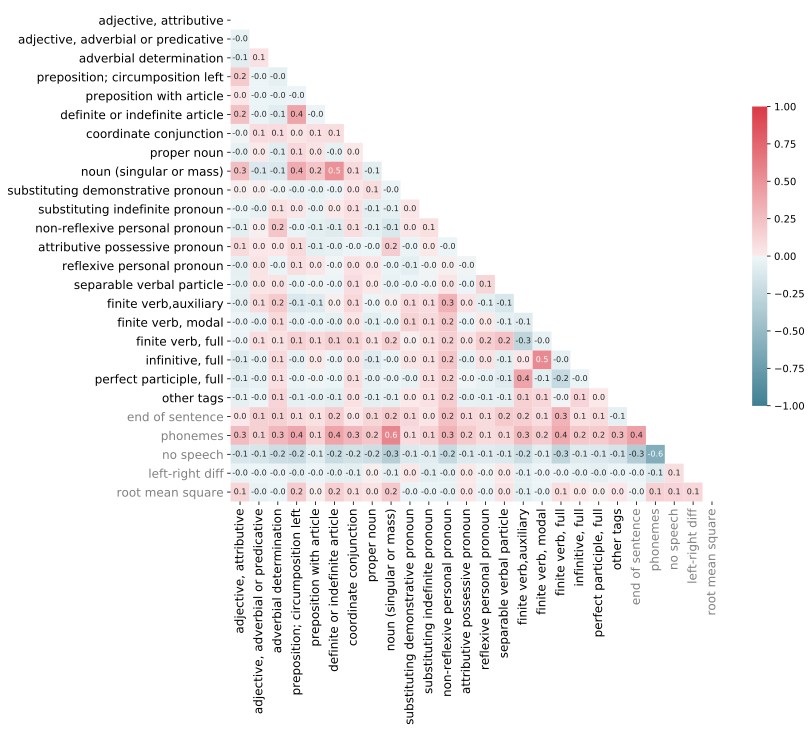
\includegraphics[width=\linewidth]{figures/regressor-corr}
  \caption{Pearson correlation coefficients of the 26 regressors used in the analysis to validate the annotation.
Regressors were convolved with FSL's ``Double-Gamma HRF'' as a model of the hemodynamic response function, temporally filtered with the same high-pass filter (cut-off 150s) as the BOLD time series, and cocatenated across runs before performing the correlation.}
\label{fig:reg-corr}
\end{figure*}


% 2nd lvl and 3rd lvl
The second-level analysis which averaged contrast estimates across the eight stimulus segments per subject was carried out using a fixed effects model by forcing the random effects variance to zero in FLAME (FMRIB's Local Analysis of Mixed Effects) \citep{beckmann2003general, woolrich2004multilevel}.
The third level analysis which averaged contrast estimates across subjects was carried out using FLAME stage 1 with automatic outlier de-weighting \citep{woolrich2004multilevel, woolrich2008robust}.
Z (Gaussianised T/F) statistic images were thresholded using clusters determined by Z>3.4 and a corrected cluster significance threshold of p<.05 \citep{woolrich2008robust}.
Brain regions associated with observed clusters were determined with the Juelich Histological Atlas \citep{eickhoff2005toolbox,eickhoff2007assignment} and the Harvard-Oxford Cortical Atlas \citep{desikan2006automated} provided by FSL.


% Results
% COPE 1:
Figure \ref{fig:results} depicts the results of the three contrasts (all Z-Threshold Z>3.4; p<.05 cluster-corrected).
The contrast words (all 21 \texttt{tag-related} regressors) > no-speech yielded four significant clusters (see Table \ref{tab:cope1}):
one left laterlized cluster spanning from the angular gyrus and inferior posterior supramarginal gyrus across the superior and middle temporal gyrus, including parts of Heschl's gyrus and planum temporale.
A second left cluster in (inferior) frontal regions, including precentral gyrus, pars opercularis (Brodman Areal 44; BA44) and pars triangularis (BA45).
Similarly in the right hemisphere, one cluster spanning from the angular gyrus across the superior and middle temporal gyrus but including frontal inferior regions (pars opercularis and pars triangularis).
A fourth significant cluster is located in the left thalamus.

% COPE 3
The contrast proper nouns > coordinate conjunctions yielded 9 significant clusters (see Table \ref{tab:cope3}):
one left laterlized cluster spanning from the angular gyrus across planum temporale and superior temporal gyrus, partially covering the Heschl's gyrus, into the anterior middle temporal gyrus.
A largely congruent but smaller cluster in the right hemisphere.
Two clusters in posterior cingulate cortex and precuneus of both hemispheres.
Three small clusters in the right occipital pole, right Heschl's gyrus and left superior lateral occipital pole.

% COPE 5
The contrast nouns > coordinate conjunctions yielded 3 significant clusters (see Table \ref{tab:cope5}):
two clusters that are slightly smaller than lateral temporal clusters of contrast nouns > coordinate conjunction. In this case, spanning from angular gyrus in the left hemisphere and from planum temporale in the right hermisphere into the anterior part of superior temporal cortex.
Finally, two small right lateralized clusters in posterior cingulate gyrus and precuneus.

\todo{Figure zeigt whole brain statt “partial brain coverage”; vgl. Text; Problem?}
\begin{figure*}
  \centering
% \includegraphics[width=0.4\textwidth]{frog.jpg}
  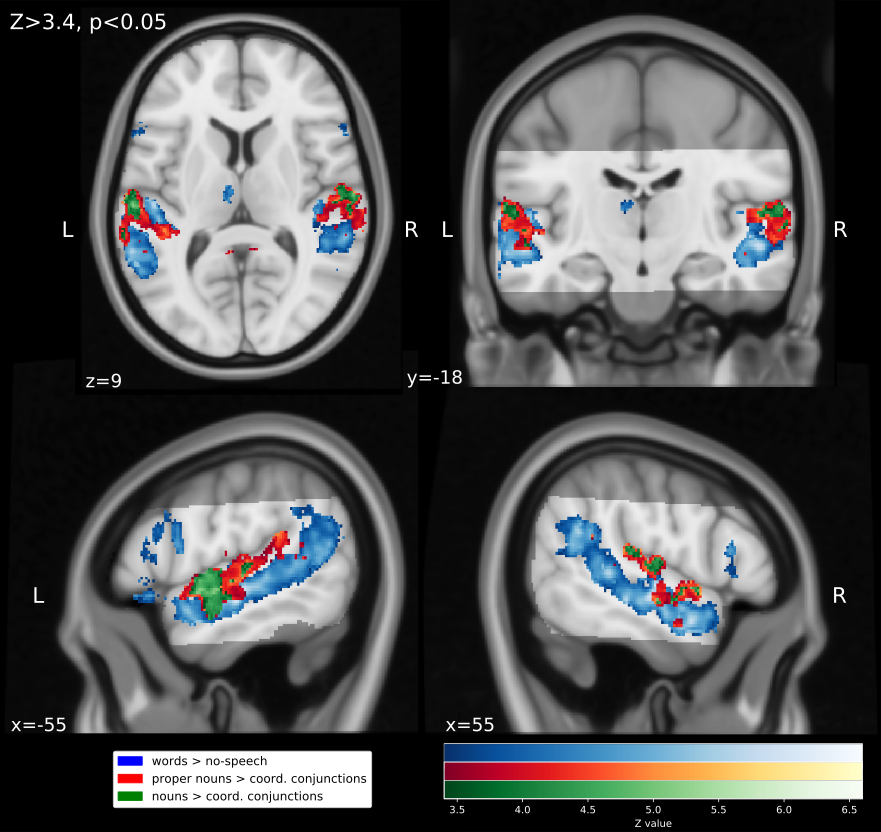
\includegraphics[width=\linewidth]{figures/slicescolorbars}
  \caption{Mixed-effects group-level (N=14) GLM contrasts for the audio-description of the movie Forrest Gump. All cluster (Z>3.4, p<0.05 cluster-corrected; MNI template space)}.
\label{fig:results}
\end{figure*}


\begin{table*}[t]
\caption{Significant clusters (Z-Threshold Z>3.4; p<.05 cluster-corrected) for the contrast words (all 21 \texttt{tag}-related regressors) > no-speech.
Clusters sorted by voxel size.
The first brain structure given contains the voxel with the maximum Z-Value, followed by brain structures from posterior to anterior, and partially covered areas.}
\label{tab:cope1}
\begin{tabular}{rrrrrrrrrp{6cm}}
\toprule
& & & \multicolumn{3}{r}{max location (MNI)} & \multicolumn{3}{r}{center of gravity (MNI)} &
\\ \cmidrule{4-6} \cmidrule{7-9}
voxels & $p_{corr.}$ & Z-max & x & y & z  & x & y & z & structure \\
\midrule
14990 & <.001 & 6.31 & -49 & -24.7 & 6.35 & -54.8 & -32.5 & 3.73 &
left Heschl's g.;
lateral superior occipital c., angular g., superior and middle temporal g. (posterior to anterior);
parts of supramarginal g. \&, planum temporale \\
14469 & <.001 & 6.48 & 55 & -14.9 & -6.9 & 54.1 & -23.1 & 0.374 &
right superior temporal g.;
angular g., superior (and middle) temporal g. (posterior to anterior), Heschl's g.;
parts of supramarginal g., planum temporale, pars opercularis (BA44) \& pars triangularis (BA45) \\
1971 & <.001 & 5.26 & -51.1 & 25.6 & -10.5 & -53.6 & 17.8 & 10.2 & left frontal orbital c.;
pars opercularis (BA44), pars triangularis (BA45);
parts of precentral g. \\
217 & .002 & 4.55 & -4.48 & -13.7 & 10.3 & -6.46 & -14.9 & 9.96 & left Thalamus \\
\bottomrule
\end{tabular}
\end{table*}


\begin{table*}[t]
\caption{Significant clusters (Z-Threshold Z>3.4; p<.05 cluster-corrected) for the contrast proper nouns (\texttt{ne}) > coordinate conjunctions (\texttt{kon}).
Clusters sorted by voxel size.
The first brain structure given contains the voxel with the maximum Z-Value, followed by brain structures from posterior to anterior, and partially covered areas.}
\label{tab:cope3}
\begin{tabular}{rrrrrrrrrp{6cm}}
\toprule
& & & \multicolumn{3}{r}{max location (MNI)} & \multicolumn{3}{r}{center of gravity (MNI)} &
\\ \cmidrule{4-6} \cmidrule{7-9}
voxels & $p_{corr.}$ & Z-max & x & y & z  & x & y & z & structure \\
\midrule
7691 & <.001 & 6.23 & -61.2 & -22.3 & 11.6 & -55.9 & -20.7 & 4.03 &
left lPanum temporale; posterior inferior supramarginal g., superior temporal g., planum polare,
parts of posterior angular g.,  Heschl's g., middle temporal gyrus \\
5928 & <.001 & 5.5 & 57.5 & -26.2 & 15.9 & 58.2 & -15.8 & 3.55 &
right planum temporale;
Heschl's g., superior temporal g., planum polare, temporal pole;
parts of angular g. \& posterior inferior supramarginal gyrus \\
479 & <.001 & 4.62 & -5.42 & -32.3 & 25.3 & -4.28 & -39.4 & 22.8 & left posterior cingulate g. \\
420 & <.001 & 4.85 & -4.76 & -71.4 & 40.1 & -3.74 & -68.5 & 36.2 & left precuneus \\
407 & <.001 & 5.07 & 6.83 & -40.1 & 24.5 & 6.67 & -38.7 & 23.1 & right posterior cingulate c. \\
294 & <.001 & 4.57 & 17 & -69.1 & 34.6 & 17.7 & -67.1 & 34.9 & right precuneus \\
121 & .024 & 3.95 & 8.12 & -98.2 & 0.359 & 8.75 & -97.7 & -3.15 & right occipital pole \\
117 & .027 & 4.38 & 36.9 & -24.8 & 4.55 & 37.4 & -23 & 3.09 & right Heschl's g. \\
115 & .029 & 4.08 & -44.6 & -71.7 & 21.7 & -43.6 & -70.8 & 23.4 & left superior lateral occipital c.\\
\bottomrule
\end{tabular}
\end{table*}


\begin{table*}[t]
\caption{Significant clusters (Z-Threshold Z>3.4; p<.05 cluster-corrected) for the contrast nouns (\texttt{nn}) > coordinate conjunctions (\texttt{kon}).
Clusters sorted by voxel size.
The first brain structure given contains the voxel with the maximum Z-Value, followed by brain structures from posterior to anterior, and partially covered areas.}
\label{tab:cope5}
\begin{tabular}{rrrrrrrrrp{6cm}}
\toprule
& & & \multicolumn{3}{r}{max location (MNI)} & \multicolumn{3}{r}{center of gravity (MNI)} &
\\ \cmidrule{4-6} \cmidrule{7-9}
voxels & $p_{corr.}$ & Z-max & x & y & z  & x & y & z & structure \\
\midrule
3166 & <.001 & 5.75 & -61.3 & -10.6 & -2.93 & -57.7 & -14.3 & 1.47 &
left anterior superior (and middle) temporal g.;
planum temporale, planum polare, anterior superior temporal g.;
part of posterior supramarginal g., Heschl's g. \\
1753 & <.001 & 4.99 & 63.3 & -15.1 & 8.41 & 58 & -13 & 4.02 & right planum temporale, anterior superior temporal g., planum polare;
part of\& part of Heschl's G. \\
166 & .004 & 4.5 & 6.83 & -40.1 & 24.5 & 7.01 & -39.7 & 24.2 &
right posterior cingulate g. \\
149 & .008 & 4.13 & 18.2 & -67.8 & 36 & 19.8 & -66.4 & 34.6 &
right precuneus \\
\bottomrule
\end{tabular}
\end{table*}

\todo[inline]{Lass uns bzgl. der Discussion am besten unterhalten; im Grunde geht es darum, wie weit ich ins Detail gehen soll (kann nämlich viel zu sehr ins Detail gehen); im Grunde geht es imo nicht darum, alle Cluster inkl. Areale durchzudiskutieren, sondern zu kommunizieren, dass die Anno brauchbar ist; wie dem auch sei: Hier wird noch Inhalt nach dem Lesen der Reviews hinzukommen}
% discussion
% wilson2007beyond
% planum temporale = Wernicke; ist witzigerweise nicht in contrast 1 (words > no speech), aber “stark” in nouns bzw. proper nouns > kon
In the contrast words > no speech, we expectedly find increased hemodynamic activity in a bilateral cortical network including temporal, parietal and frontal regions realted to processing spoken language \citep{friederici2011brain, hickok2007cortical,price2012twentyyears}.\todo{abchecken}
Our results are similar to results of studies that implemented an ISC approach to analyze fMRI data of naturalistic auditory stimuli \citep{honey2012not, lerner2011topographic, silbert2014coupled}.
Contrary to previous studies, we do not find increased medial activation in the precuneus or medial frontal cortex. This could be attributed to the fact that our contrast does not [+++sufficiently+++] capture social aspects of the narrative \citep{ferstl2008extended, mar2011neural}\todo{abchecken}.
The two contrasts contrasting nouns and proper nouns respectively to coordinate junctions lead to unexpected results. Increased activation is partially located in early sensory regions (Heschl's Gyrus; \citep{saenz2014tonotopic}) and most prominently adjacant regions bilaterally (planum temporale; superior temporal gyrus; \citep{arsenault2015distributed, mesgarani2014phonetic}).
This could be attributed to the fact that a high count of heterogenous nouns (N=\rNnAll) and proper nouns (N=\rNeAll) were averaged across all 300 semantic dimensions (cf. \citep{mitchell2008predicting, huth2016natural}), and contrasted to coordinate conjunctions that offered a comparably small amount of events (N=\rKonAll).
Moreover, the coordinate junctions (\texttt{kon}) mostly comprises event of the words ``and'' (N=392) and ``but'' (N=49) and thus offered only a small amount of variance.
A second explanation might be that our phoneme regressors that assumed linear summation of approximatly 70 ms lasting events in quick succession did not capture a sufficiently amount of nuissance variance.
Nevertheless and more importantly to access the validity of the dataset is the fact that two similar lingustic concepts (nouns and proper nouns) embedded in a naturalistic stimulus that was not designed for linguistic research lead to similar activation patterns.
% Within the language processing systems, early sensory regions are specialized for representing the immediate physical properties of the environment (form), while higher order regions extract increasingly abstract content (Davis and Johnsrude, 2003; Quiroga et al., 2005; Okada et al., 2010).

\section*{Data availability}
% aus der Schnitt-Annotation übernommen
\texttt{This section will be auto-generated.}

In addition, released data, code, and manuscript sources are also available on
Github (\url{https://github.com/psychoinformatics-de/studyforrest-paper-speechannotation}).

\section*{Conclusions}
\todo[inline]{the paper needs to serve a purpose.
One is, of course, to be documentation for the annotation.
Another is to attract people to use this work for their own studies.
I would even argue that this is the \textit{main} purpose, given that the annotation in itself represents to scientific progress.
The need to give an accurate assessment what this can be used for and what is problematic or impossible.
ATM this is the only statement in this regard:
'facilitates modelling of hemodynamic brain responses correlating with speech-related events' and the only indication of purpose is 'additional confound measures'.
I think this is incongruent with the amount of work and the level of detail of
this annotation; öööööhh, okay. Mir sind da jetzt über 2 Tage wenig Superlative eingefallen, die über den bisherigen Text hinausgehen; fehlt mir wohl die geeignete Perspektive}
% state what you think are the main conclusions that can be realistically drawn from the findings in the paper, taking care not to make claims that cannot be supported.
As an extension of the studoforrest dataset, we present an annotation of spoken language in the two hours lasting ``research cut'' of the audio-visual movie ``Forrest Gump'' and its temporally aligned audio-description.
We annotated the onset and offset of sentences, words and phonemes, and the corresponding speaker's identity.
An additional tagging of each word's linguistic features and the public nature of the dataset enable independent working groups to create sophisticated models of hemodynamic activity correlating with speech-related events in a naturalistic stimulus.
Results of our dataset validating analysis that we run as a proof of concept show that the annotation's content can indeed / in principle be used to isolate/track speech-related networks in the human brain under life-like conditions.


\subsection*{Author contributions}
% subsection in Schnitte-Anno
%In order to give appropriate credit to each author of an article, the
%individual contributions of each author to the manuscript should be detailed
%in this section. We recommend using author initials and then stating briefly
%how they contributed.
COH designed, performed, and validated the annotation, and wrote the manuscript.
MH provided critical feedback on the procedure and wrote the manuscript.

\subsection*{Competing interests}
% subsection in Schnitte-Anno
No competing interests were disclosed.

\subsection*{Grant information}

COH was supported by a graduate stipend from the German federal state of
Saxony-Anhalt and MH was supported by funds from the German federal state of
Saxony-Anhalt and the European Regional Development Fund (ERDF), Project:
Center for Behavioral Brain Sciences (CBBS). Work on the adapting data
management technology for this study was in part supported by the European
Union's Horizon 2020 Research and Innovation Programme under Grant Agreement
no. 785907 (HBP SGA2).


\subsection*{Acknowledgements}
We are grateful to \href{www.florianschurz.de}{Florian Schurz} who initiated doing the annotation of the descriptive nouns\todo{should it still be here? or move in PPA paper?}, and performed the preliminary annotation of nouns. Christian O. Häusler is also grateful to Valeri Kippes who took care of the author's mental sanity by providing excellent training at his gym in Jülich during the mentally draining period of manual corrections of the annotation.

{\small\bibliographystyle{unsrtnat}
\bibliography{references}}

\end{document}
